\chapter{Thiết kế Mạch nguyên lý và PCB Layout (Schematic and PCB Layout Design)}
    \section{Thiết kế Mạch nguyên lý (Schematic Design)}
        Phần này trình bày các nội dung kỹ thuật của dự án thông qua thiết kế sơ đồ nguyên lý. Thiết kế sơ đồ nguyên lý mô tả chi tiết các kết nối điện giữa các thành phần, nhằm đảm bảo hệ thống hoạt động đúng chức năng, đồng thời đáp ứng các yêu cầu về hiệu năng và các ràng buộc trong thiết kế.

        \begin{figure}[h]
            \centering
            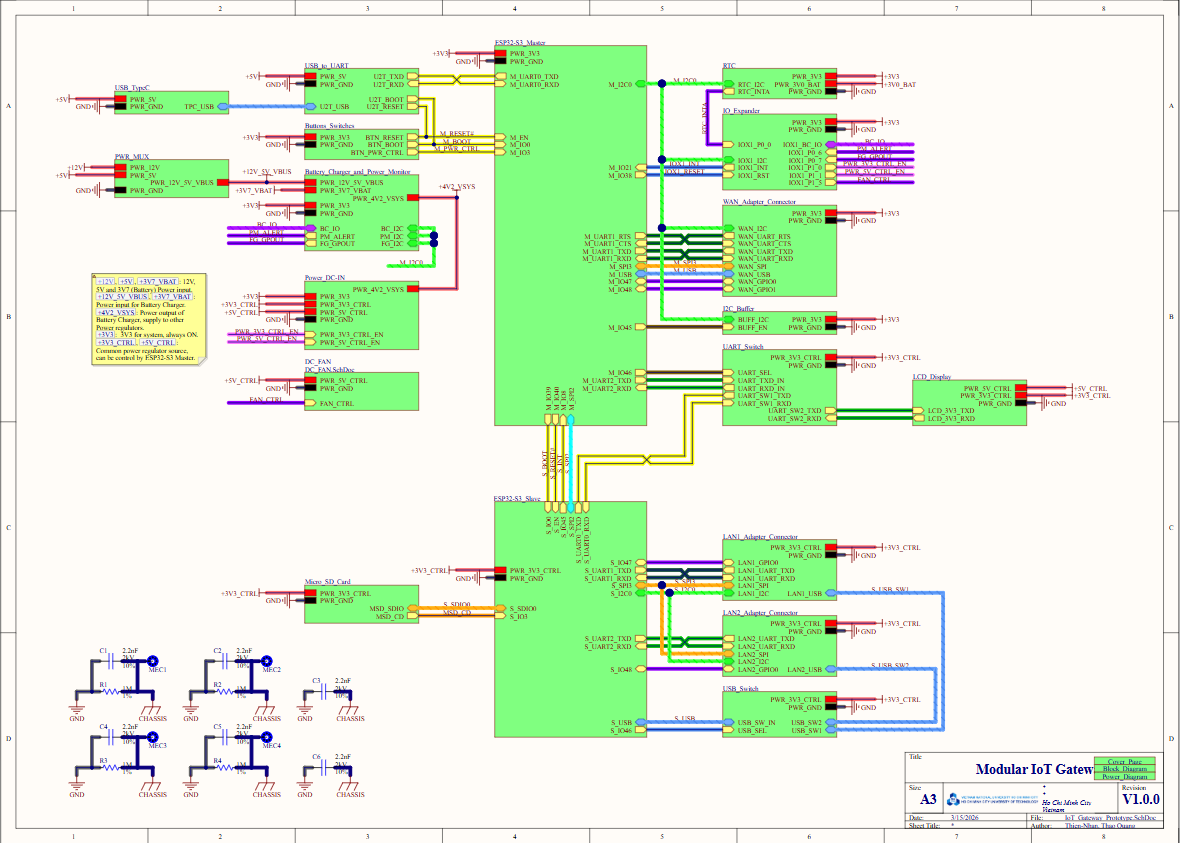
\includegraphics[width=0.75\textwidth]{figures/DATN/sche_iotgateway.png}
            \caption{Sơ đồ nguyên lý hệ thống}
            \label{fig:sche_iotgateway}
        \end{figure}

        % Nội dung mục này đã được chuyển lên Chương 4, mục 4.3.1 (Thiết kế Mạch xử lý trung tâm).

        \subsection{Thiết kế Mạch nguồn}

            % IC Power MUX TPS2121RUXR tiếp nhận hai nguồn đầu vào chính, bao gồm +12V (từ adapter) và +5V (từ cổng USB). Tại mỗi đầu vào, hệ thống tích hợp một diode TVS với điện áp Reverse Standoff tương ứng với mức điện áp danh định của từng nguồn. Linh kiện này có chức năng hấp thụ và triệt tiêu năng lượng của các xung điện áp ngắn hạn (ESD), qua đó bảo vệ khối nguồn và các thành phần phía sau khỏi ảnh hưởng của hiện tượng phóng tĩnh điện hoặc nhiễu xung điện áp cao từ môi trường.
            IC Power MUX TPS2121RUXR tiếp nhận hai nguồn đầu vào chính, bao gồm +12V (từ adapter) và +5V (từ cổng USB). Mạch tích hợp diode TVS tại các ngõ vào +12V và +5V của IC TPS2121RUXR giúp bảo vệ hệ thống trước các rủi ro tĩnh điện. Giải pháp này triệt tiêu xung ESD tức thời, bảo đảm tính toàn vẹn cho khối nguồn và các linh kiện nhạy cảm nguồn trước nhiễu điện áp cao từ môi trường.

            \begin{figure}[h]
                \centering
                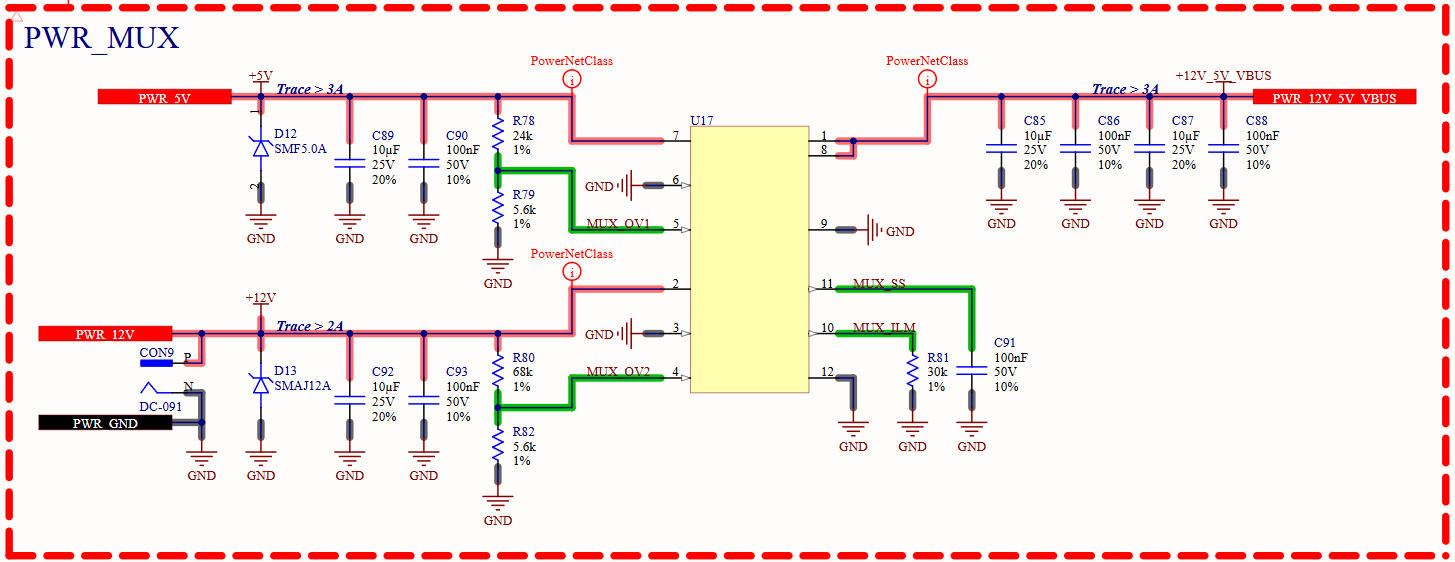
\includegraphics[width=0.75\textwidth]{figures/DATN/sche_powermux.png}
                \caption{Sơ đồ nguyên lý mạch Power MUX}
                \label{fig:sche_powermux}
            \end{figure}

            Các thông số thiết kế cho IC Power MUX TPS2121RUXR được lựa chọn như sau:

            \begin{itemize}
                \item Điện áp bảo vệ quá áp (overvoltage) đối với nguồn +5V (USB): 5.6V;
                \item Điện áp bảo vệ quá áp đối với nguồn +12V (adapter): 13.93V;
                \item Giới hạn dòng điện đầu vào tối đa: 3.49A;
                \item Thời gian khởi động mềm (soft-start) khi kết nối nguồn +5V: 6.41ms;
                \item Thời gian khởi động mềm khi kết nối nguồn +12V: 15ms.
            \end{itemize}
            Các tham số trên được lựa chọn nhằm đảm bảo quá trình chuyển mạch nguồn diễn ra ổn định, hạn chế dòng xung khởi động, đồng thời tăng cường khả năng bảo vệ và độ tin cậy cho toàn bộ hệ thống.

            Nguồn sau Power MUX cùng với nguồn dự phòng từ pin LiPo được đưa vào và quản lý bởi IC sạc BQ25892RTWR. Dòng đầu vào của IC được giới hạn ở mức 2.96A thông qua điện trở cấu hình tại chân ILIM. Các giá trị tụ điện ở đầu vào và đầu ra được lựa chọn theo khuyến nghị nhằm đảm bảo ổn định điện áp và giảm nhiễu trong quá trình vận hành.\cite{FastChargerBq2589x}

            \begin{figure}[h]
                \centering
                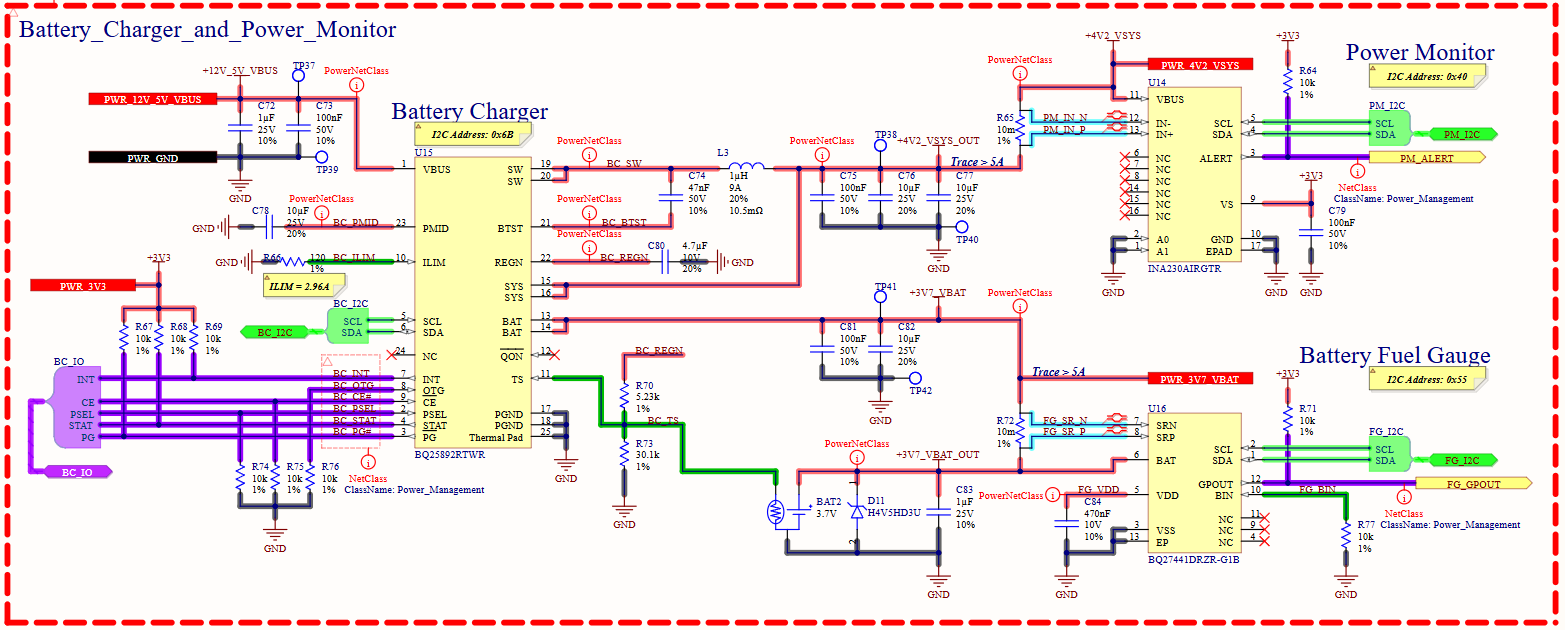
\includegraphics[width=0.75\textwidth]{figures/DATN/sche_batterycharger.png}
                \caption{Sơ đồ nguyên lý mạch sạc, quản lý pin LiPo và giám sát công suất}
                \label{fig:sche_batterycharger}
            \end{figure}

            Dòng sạc tối đa của hệ thống được thiết kế với $I_{CHG} = 5A$, dòng bão hòa của cuộn cảm phải thỏa mãn điều kiện\cite{FastChargerBq2589x}:

            \begin{equation}
            I_{SAT} \geq I_{CHG} + \dfrac{1}{2} I_{RIPPLE}
            \end{equation}

            Trong đó, dòng ripple của cuộn cảm được xác định bởi:

            \begin{equation}
            I_{RIPPLE} = \dfrac{V_{BUS} \times D \times (1 - D)}{f_s \times L}
            \end{equation}

            Với các tham số thiết kế: $V_{BUS} = 12V$, $D = 0.5$ (trường hợp xấu nhất), $f_s = 1.5\,MHz$ và $L = 1\,\mu H$, suy ra $I_{RIPPLE} \approx 2A$

            Từ đó, yêu cầu dòng bão hòa tối thiểu của cuộn cảm $I_{SAT\_req} \geq 5A + \frac{1}{2} \times 2A = 6A$

            Lựa chọn cuộn cảm MDA5030-1R0M ($I_{SAT_typ} = 8.5A$) thiết lập biên độ dự phòng 30-50\% so với tính toán, giúp giảm thiểu rủi ro từ sai số linh kiện và bảo đảm khối nguồn vận hành ổn định. Pin LiPo tích hợp sẵn mạch bảo vệ và NTC 10k, đảm bảo an toàn và tin cậy khi vận hành thiết bị.

            Trong quá trình vận hành, điện áp đầu ra VSYS của IC sạc có thể thay đổi tùy theo trạng thái cấp nguồn của hệ thống, cụ thể như sau:
            \begin{itemize}
                \item \textbf{Chỉ có nguồn VBUS (5V từ USB hoặc 12V từ adapter):} 
                Kiến trúc Narrow VDC duy trì VSYS ở khoảng 3.65V ổn định ngay cả khi thiếu pin, bảo đảm hệ thống vận hành liên tục và giảm rủi ro sụt áp.

                \item \textbf{Chỉ cấp nguồn từ VBAT (mất hoặc không kết nối VBUS):} 
                Duy trì VSYS trong ngưỡng 3.5V - 4.2V, bảo vệ pin khỏi hiện tượng xả sâu, đồng thời bảo đảm biên độ điện áp ổn định cho các khối nguồn hạ nguồn vận hành tin cậy.

                \item \textbf{Cấp nguồn đồng thời từ VBUS và VBAT (trạng thái sạc):}
                Trong trường hợp này, điện áp VSYS phụ thuộc vào mức điện áp pin:
                \begin{itemize}
                    \item Khi điện áp pin thấp (từ 3.0\,V đến dưới 3.5\,V): 
                    BATFET hoạt động ở chế độ tuyến tính (LDO mode) để duy trì điện áp hệ thống lớn hơn điện áp pin. VSYS được giữ ổn định tại mức $VSYS(MIN) + 150\,mV$, tương đương khoảng 3.65\,V.

                    \item Khi điện áp pin lớn hơn 3.5\,V: 
                    BATFET được bật hoàn toàn, điện áp VSYS sẽ bám theo điện áp pin với độ lệch khoảng 50\,mV, tức là $VSYS \approx VBAT + 50\,mV$. Do đó, VSYS tăng dần trong khoảng từ 3.55\,V đến 4.25\,V.

                    \item Trường hợp quá tải (chế độ Supplement): 
                    Khi dòng tải vượt khả năng cung cấp của VBUS, điện áp VSYS có xu hướng giảm. Khi VSYS thấp hơn điện áp pin, IC sẽ chuyển sang sử dụng năng lượng từ pin để bổ sung cho hệ thống. Khi đó, VSYS xấp xỉ bằng điện áp pin, nằm trong khoảng từ 3.5\,V đến 4.2\,V.
                \end{itemize}
            \end{itemize}

            Việc tích hợp IC INA230AIRGTR tại đầu ra VSYS cho phép giám sát công suất toàn hệ thống theo thời gian thực với sai số thấp (tối đa 0.3\%). Lựa chọn này đảm bảo dữ liệu năng lượng tin cậy mà không gây hao tổn đáng kể nhờ dòng tiêu thụ thấp (tối đa 420 $\mu$A). Song song đó, IC BQ27441DRZR-G1B được sử dụng để quản lý trạng thái pin LiPo, hoàn thiện giải pháp giám sát năng lượng đồng bộ cho thiết bị.

            \begin{figure}[h]
                \centering
                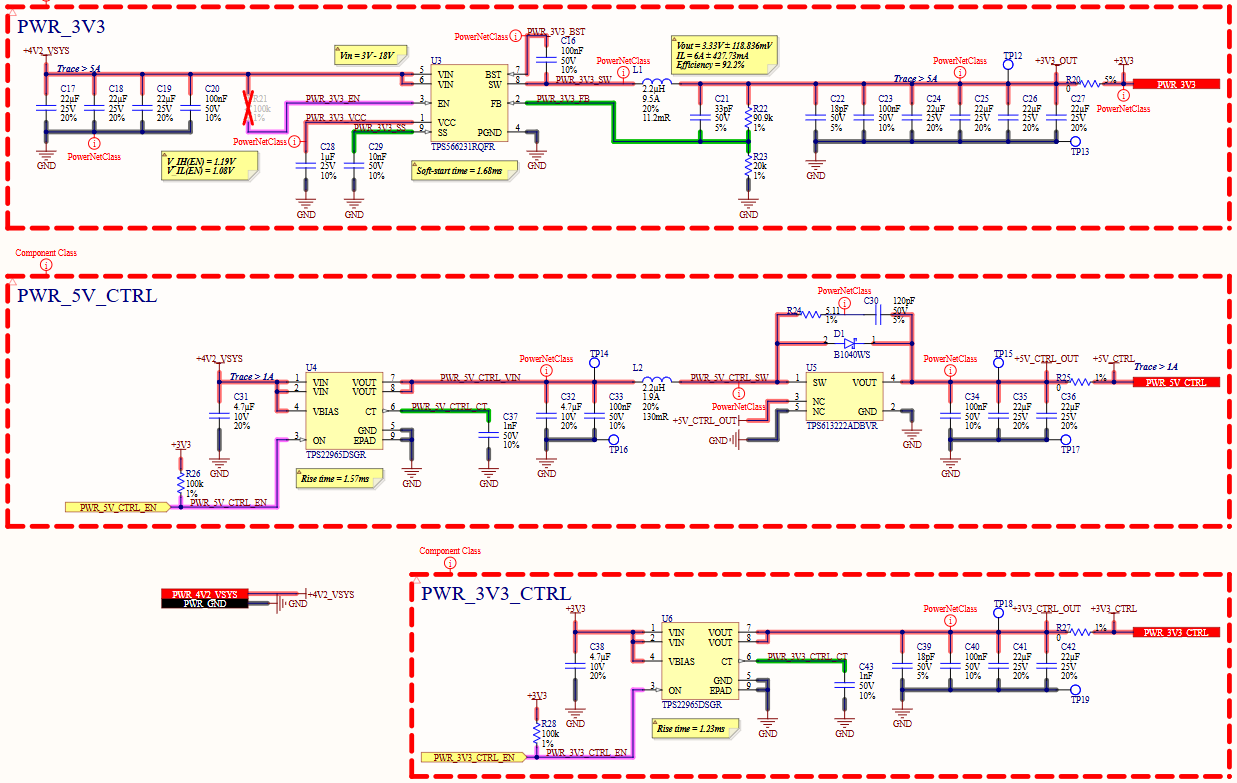
\includegraphics[width=0.75\textwidth]{figures/DATN/sche_powerdcdc.png}
                \caption{Sơ đồ nguyên lý mạch nguồn DC-DC}
                \label{fig:sche_powerdcdc}
            \end{figure}

            Các tụ điện đầu vào được lựa chọn theo khuyến nghị của nhà sản xuất, với điện áp định mức tối thiểu lớn hơn hai lần điện áp làm việc nhằm đảm bảo độ tin cậy. Cuộn cảm được chọn với khả năng chịu dòng DC cao hơn khoảng 30--50\% so với giá trị tính toán, giúp duy trì hoạt động ổn định trong điều kiện tải biến thiên.

            Các cấu hình thiết kế chi tiết trên nền tảng WEBENCH TI như sau:
            \begin{itemize}
                \item \textbf{PWR\_3V3:} \href{https://webench.ti.com/appinfo/webench/scripts/SDP.cgi?ID=A65948A5E7EE6E50}{TPS566231RQFR -- 3.5V--4.2V to 3.30V @ 5A};
                \item \textbf{PWR\_5V\_CTRL:} \href{https://webench.ti.com/appinfo/webench/scripts/SDP.cgi?ID=07E521FCC698EE21}{TPS613222ADBVR -- 3.5V--4.2V to 5.00V @ 0.5A}.
            \end{itemize}

            Các khối nguồn điều khiển PWR\_3V3\_CTRL và PWR\_5V\_CTRL được thiết kế với đầu vào đi qua IC power switch TPS22965DSGR. Mặc định, các kênh nguồn này ở trạng thái bật (ON) và có thể được điều khiển đóng/ngắt thông qua IO Expander do MCU master quản lý.

            Các rail nguồn cấp cho các thành phần trong hệ thống được cấu hình với thời gian khởi động mềm (soft-start) tối thiểu lớn hơn 1\,ms, nhằm hạn chế dòng khởi động đột ngột (inrush current) và đảm bảo tính ổn định trong quá trình cấp nguồn.  

        \subsection{Thiết kế Mạch USB và USB to UART Bridge}

            Cổng USB có thể sử dụng để cung cấp nguồn cho hệ thống, đồng thời hỗ trợ cấu hình thiết bị và nạp firmware trong quá trình phát triển và vận hành.
            
            Giao diện USB tích hợp bảo vệ ESD qua TVS diode H5VUD5BB trên hai đường dữ liệu, vừa đảm bảo an toàn vận hành, vừa duy trì toàn vẹn tín hiệu nhờ điện dung ký sinh cực thấp 0.3 pF tại 1\,MHz, đảm bảo tốc độ truyền chuẩn Full-Speed 12\,Mbit/s, giảm thiểu suy hao biên độ hay méo dạng sóng.

            \begin{figure}[h]
                \centering
                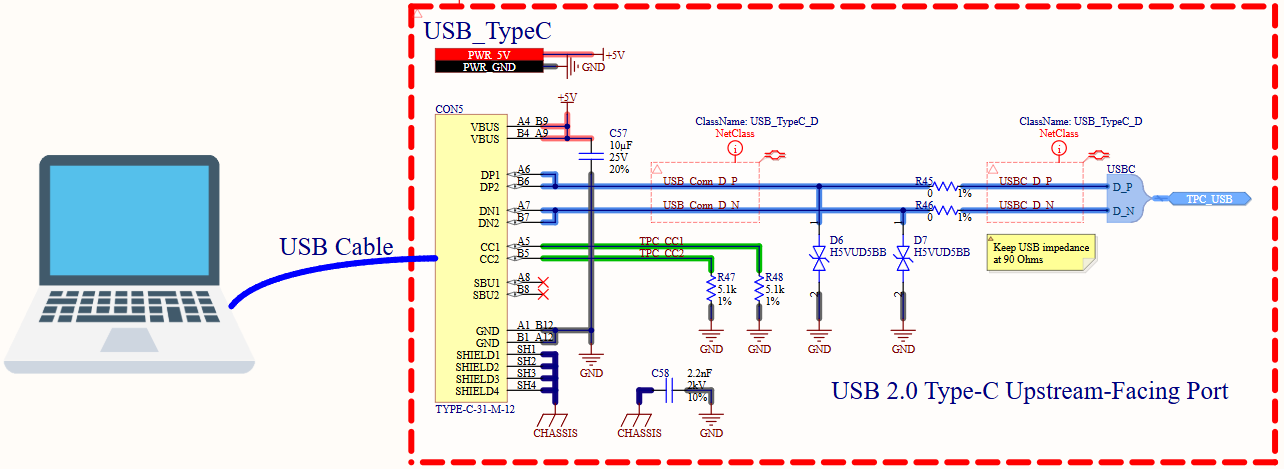
\includegraphics[width=0.75\textwidth]{figures/DATN/sche_usbconn.png}
                \caption{Sơ đồ nguyên lý mạch USB}
                \label{fig:sche_usbconn}
            \end{figure}

            Ngoài ra, trên mỗi đường D$^+$ và D$^-$ còn được bố trí thêm điện trở giảm chấn (series damping resistor) 22\,$\Omega$\cite{EngineersGuideToUsbTypeC}\cite{UsbTypeCCableConnectorSpecification}, với tác dụng:
            \begin{itemize}
                \item Giảm hiện tượng overshooting và ringing trên cạnh xung
                \item Cải thiện Signal Integrity
                \item Giảm phát xạ EMI (Electromagnetic Interference)
            \end{itemize}
            
            Thiết bị sử dụng IC USB-to-UART Bridge CP2102-GMR để thực hiện chuyển đổi giao tiếp từ USB sang UART, kết nối trực tiếp với UART0 của ESP32-S3 Master. Khối này phục vụ cho việc nạp firmware, cấu hình thiết bị trong quá trình phát triển và vận hành.

            \begin{figure}[H]
                \centering
                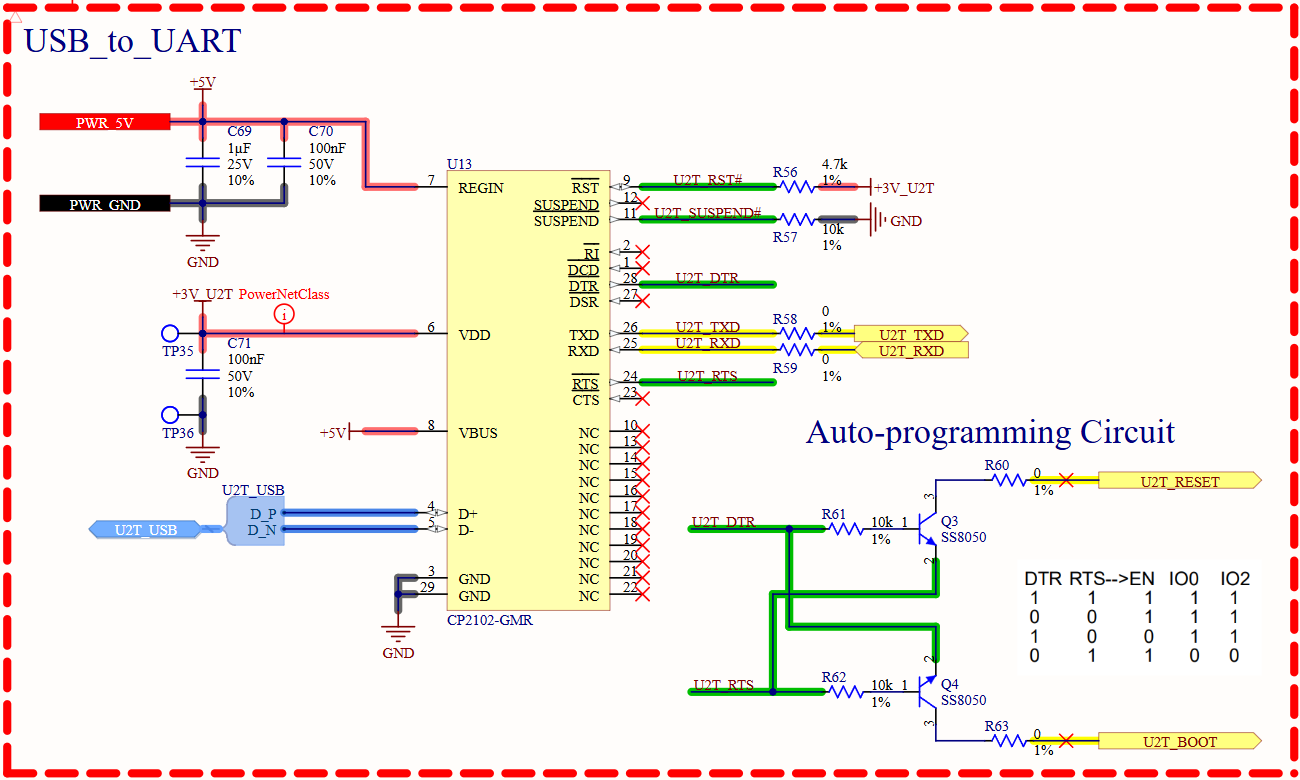
\includegraphics[width=0.75\textwidth]{figures/DATN/sche_usb2uartbridge.png}
                \caption{Sơ đồ nguyên lý mạch USB to UART Bridge}
                \label{fig:sche_usb2uartbridge}
            \end{figure}

            Các tín hiệu điều khiển DTR và RTS từ IC được khai thác và tích hợp vào mạch auto-programming thông qua hai transistor BJT NPN. Mạch này cho phép tự động điều khiển các tín hiệu Reset và Boot của ESP32-S3 Master, hỗ trợ quá trình nạp firmware mà không cần thao tác thủ công thông qua các nút nhấn Reset và Boot.

        \subsection{Thiết kế Mạch IO Expanders}
            Mạch tích hợp IC TCA6416ARTWR qua I2C giúp mở rộng 16 chân GPIO, đảm bảo hệ thống đáp ứng đầy đủ nhu cầu kết nối ngoại vi phức tạp. Lựa chọn này hỗ trợ tính linh hoạt trong thiết kế khi cho phép cấu hình tùy biến ngõ vào/ra cho từng kịch bản vận hành.

            \begin{figure}[h]
                \centering
                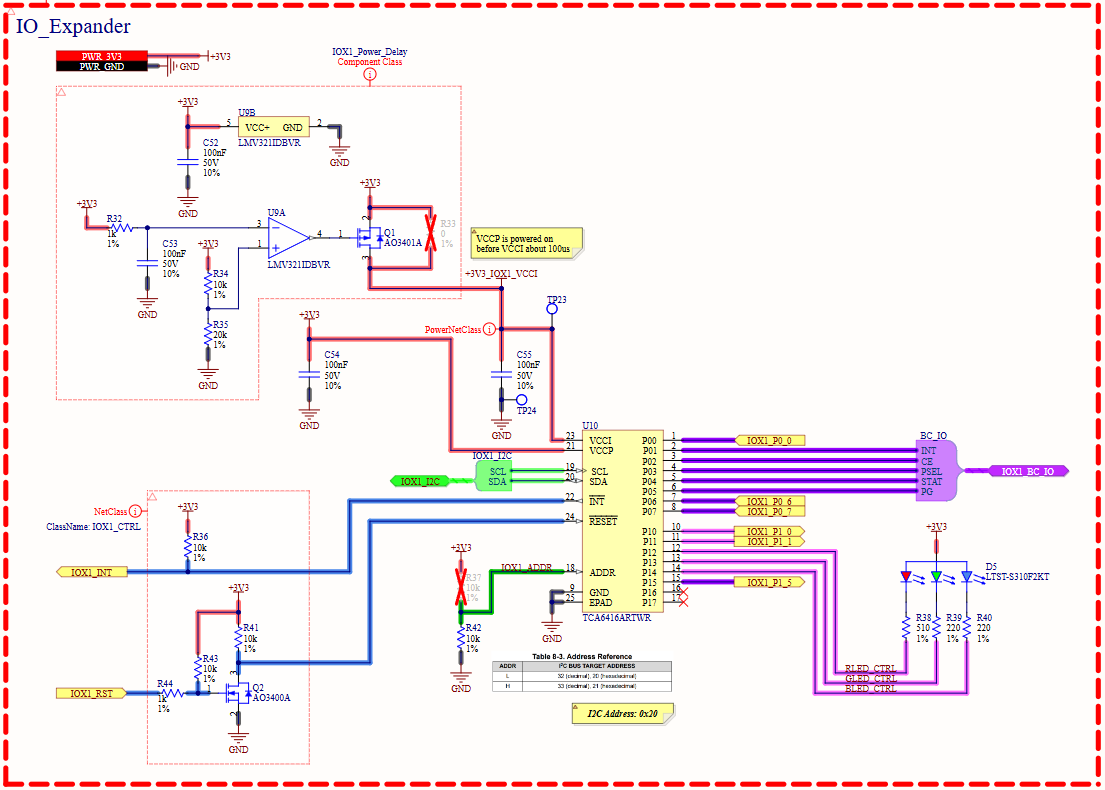
\includegraphics[width=0.75\textwidth]{figures/DATN/sche_ioexpanders.png}
                \caption{Sơ đồ nguyên lý mạch IO Expanders} 
                \label{fig:sche_ioexpanders}
            \end{figure}
            
            Nhằm ngăn ngừa lỗi kẹt bus SDA, thiết kế tích hợp mạch delay tại chân VCCI để đảm bảo trình tự VCCP cấp trước VCCI (>0.1 ms)\cite{IoExpanderTca6416a}. Việc tuân thủ đặc tả kỹ thuật này đảm bảo tính ổn định của hệ thống ngay từ giai đoạn khởi động, đáp ứng yêu cầu vận hành tin cậy của IC IO Expander.

            \begin{figure}[H]
                \centering
                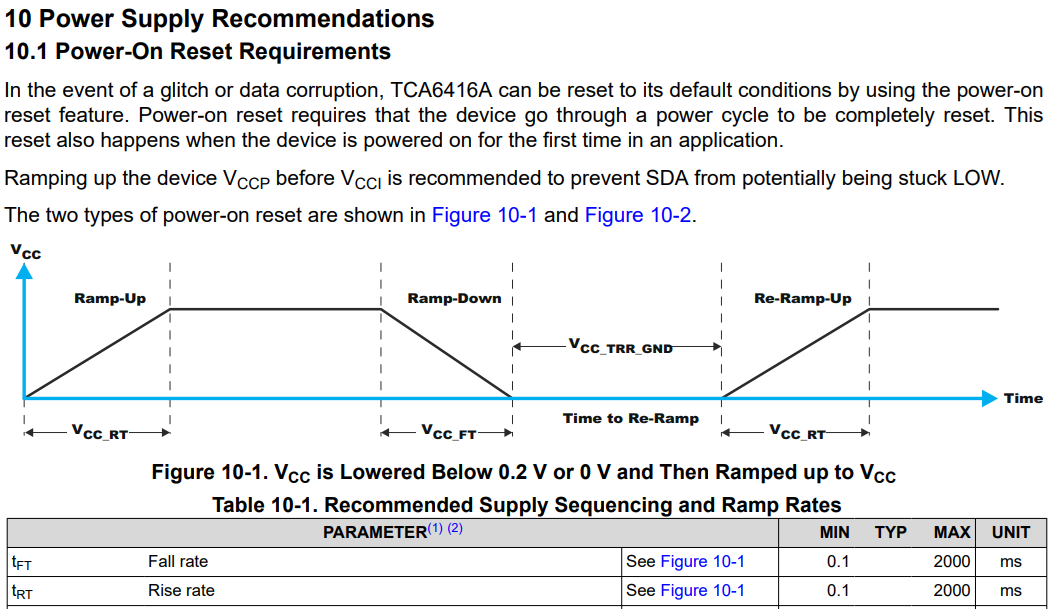
\includegraphics[width=0.5\textwidth]{figures/DATN/datasheet_ioxpowerrecomendation.png}
                \caption{Khuyến nghị cấp nguồn cho IC TCA6416ARTWR từ datasheet} 
                \label{fig:sche_ioxpowerrecomendation}
            \end{figure}

            Tại đầu vào dương của bộ so sánh là một cầu chia áp nhằm tạo điện áp tham chiếu. Điện áp tham chiếu này có giá trị xấp xỉ 2.2\,V. Tại đầu vào âm của bộ so sánh là mạch RC delay, trong đó điện áp trên tụ tăng dần theo thời gian khi mạch được cấp nguồn. Khi điện áp trên tụ vượt qua mức tham chiếu 2.2\,V, đầu ra của bộ so sánh sẽ chuyển từ mức thấp sang mức cao, kích hoạt MOSFET kênh P đóng và cấp nguồn cho chân VCCI của IO Expander.

            Với các giá trị được lựa chọn trong thiết kế, trong đó $\tau = RC = 0.1\,\text{ms}$, điện áp nguồn $V_S = 3.3\,\text{V}$ và điện áp trên tụ tại thời điểm so sánh $V_C = 2.2\,\text{V}$, thời gian trễ tính toán được là $t \approx \textbf{0.11\,ms}$. Giá trị này đáp ứng dải thời gian ramp-up từ 0.1 đến 2000\,ms theo khuyến nghị trong datasheet của nhà sản xuất.

            Cơ chế hoạt động của mạch được mô tả theo trình tự thời gian như sau:
            \begin{itemize}
                \item \textbf{Tại thời điểm $t = 0$}: mạch IO Expander vừa được cấp nguồn. Điện áp tại đầu vào âm của bộ so sánh bắt đầu tăng dần từ 0\,V lên mức 3.3\,V, trong khi điện áp tại đầu vào dương được giữ cố định ở mức 2.2\,V. Op-amp cho mức điện áp đầu ra cao (xấp xỉ 3.3\,V), khiến MOSFET kênh P ở trạng thái đóng, nguồn VCCI chưa được cấp.
                \item \textbf{Tại thời điểm $t \approx 0.11\,ms$}: điện áp tại đầu vào âm vượt qua mức 2.2\,V, làm đầu ra op-amp bị kéo xuống mức thấp (xấp xỉ 0\,V). MOSFET kênh P chuyển sang trạng thái dẫn, cho phép nguồn VCCI được cấp cho IO Expander.
            \end{itemize}

            Mạch được mô phỏng trên phần mềm LTspice, kết quả mô phỏng được trình bày trong Hình~\ref{fig:sim_ioxdelayvcci}.

            \begin{figure}[H]
                \centering
                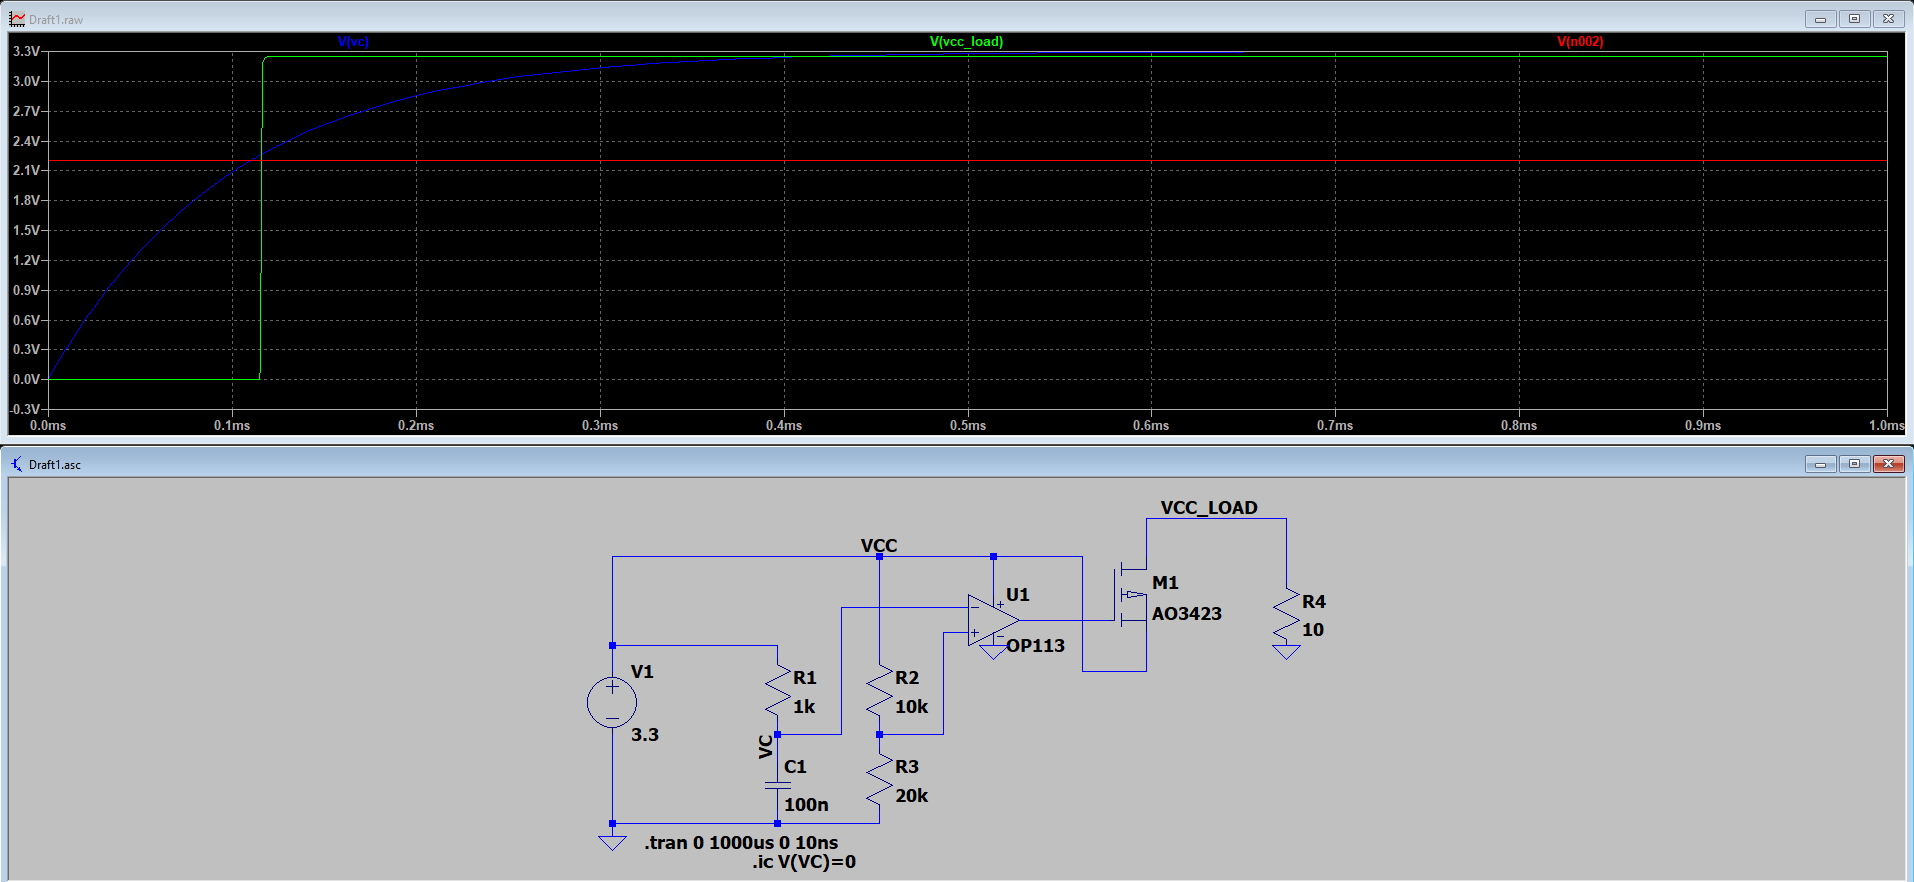
\includegraphics[width=0.85\textwidth]{figures/sim_ioxdelayvcci.png}
                \caption{Kết quả mô phỏng mạch delay khởi động nguồn VCCI cho IO Expander} 
                \label{fig:sim_ioxdelayvcci}    
            \end{figure}

        \subsection{Thiết kế Mạch RTC}
            Hệ thống tích hợp IC PCF8563 (I2C) cùng mạch Power OR-ing dùng diode Schottky nhằm đảm bảo dữ liệu thời gian thực được duy trì thông suốt trong mọi tình huống chuyển đổi nguồn. Việc bố trí diode TVS tại đường pin dự phòng là giải pháp cần thiết để triệt tiêu xung ESD, bảo vệ mạch khỏi rủi ro hỏng hóc khi thay pin. Việc sử dụng thạch anh 32.768kHz có ESR < 100\,k$\Omega$ và điện dung 12.5pF là sự tuân thủ yêu cầu của IC, giúp hệ thống đạt độ chính xác cao nhất và tối ưu hóa năng lượng vận hành.
            \begin{figure}[H]
                \centering
                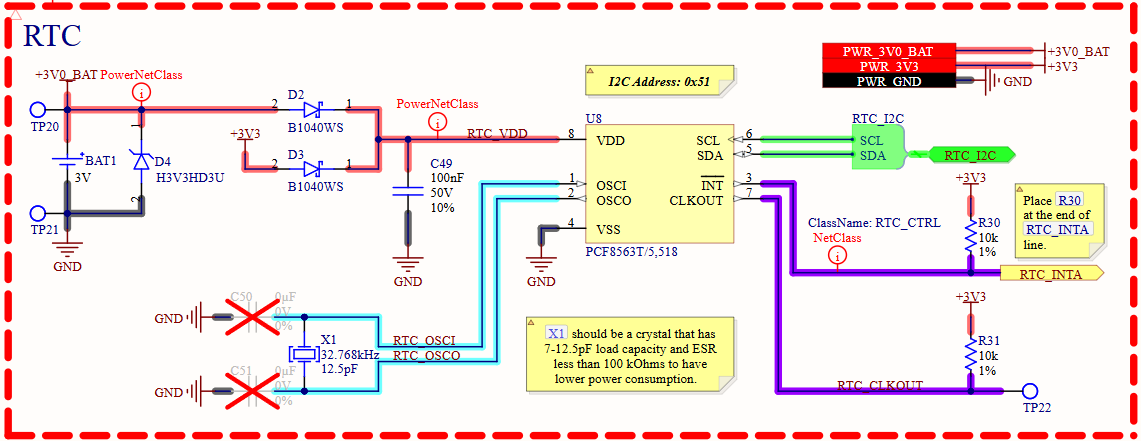
\includegraphics[width=0.75\textwidth]{figures/DATN/sche_rtc.png}
                \caption{Sơ đồ nguyên lý mạch RTC} 
                \label{fig:sche_rtc}
            \end{figure}

        \subsection{Thiết kế Mạch Micro SD Card}
            Giao tiếp thẻ MicroSD được thực hiện qua chuẩn SDIO 4-bit (80MHz) nhằm đảm bảo thông lượng lưu trữ dữ liệu tối ưu cho hệ thống. Để triệt tiêu hiện tượng ringing và overshoot phát sinh ở tần số cao, thiết kế tuân thủ nghiêm ngặt khuyến nghị của Espressif bằng cách tích hợp IC EMIF06-MSD02N16 ngay tại ngõ vào. Việc sử dụng linh kiện chuyên dụng này không chỉ giúp tối ưu hóa diện tích bo mạch mà còn là giải pháp kỹ thuật đồng bộ, cung cấp đồng thời trở giảm chấn (36-54\,$\Omega$), điện trở kéo lên (80-100k\,$\Omega$) và tầng bảo vệ ESD, giúp duy trì tính toàn vẹn tín hiệu vượt trội so với việc sử dụng các linh kiện rời rạc.


            \begin{figure}[h]
                \centering
                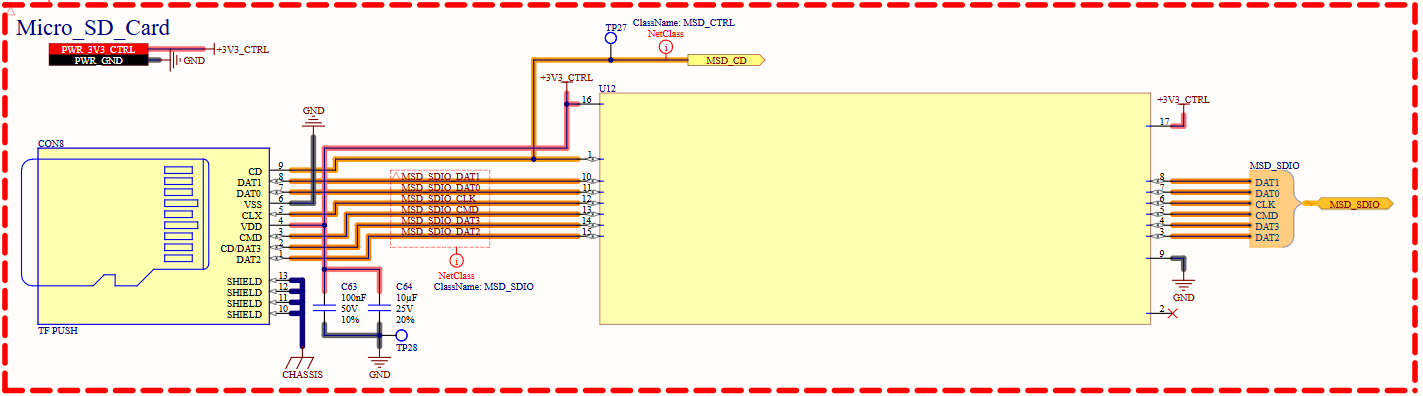
\includegraphics[width=0.75\textwidth]{figures/DATN/sche_microsd.png}
                \caption{Sơ đồ nguyên lý mạch Micro SD Card} 
                \label{fig:sche_microsd}
            \end{figure}

        \subsection{Thiết kế Mạch USB/UART Switch}
            Nhằm khắc phục giới hạn duy nhất một giao diện USB vật lý trên ESP32-S3, thiết kế tích hợp IC FSUSB42UMX-TP làm giải pháp điều phối tín hiệu chủ động. Việc sử dụng switch analog này cho phép hệ thống chuyển mạch linh hoạt giữa các đầu nối LAN hoặc giao tiếp UART, đảm bảo Gateway vận hành đa nhiệm mà không cần tăng số lượng nhân xử lý. Lựa chọn linh kiện chuyên dụng này giúp duy trì tính toàn vẹn tín hiệu USB Host, đồng thời đáp ứng yêu cầu về một kiến trúc phần cứng tinh gọn nhưng vẫn có khả năng mở rộng cao theo nhu cầu thực tế.

            \begin{figure}[h]
                \centering
                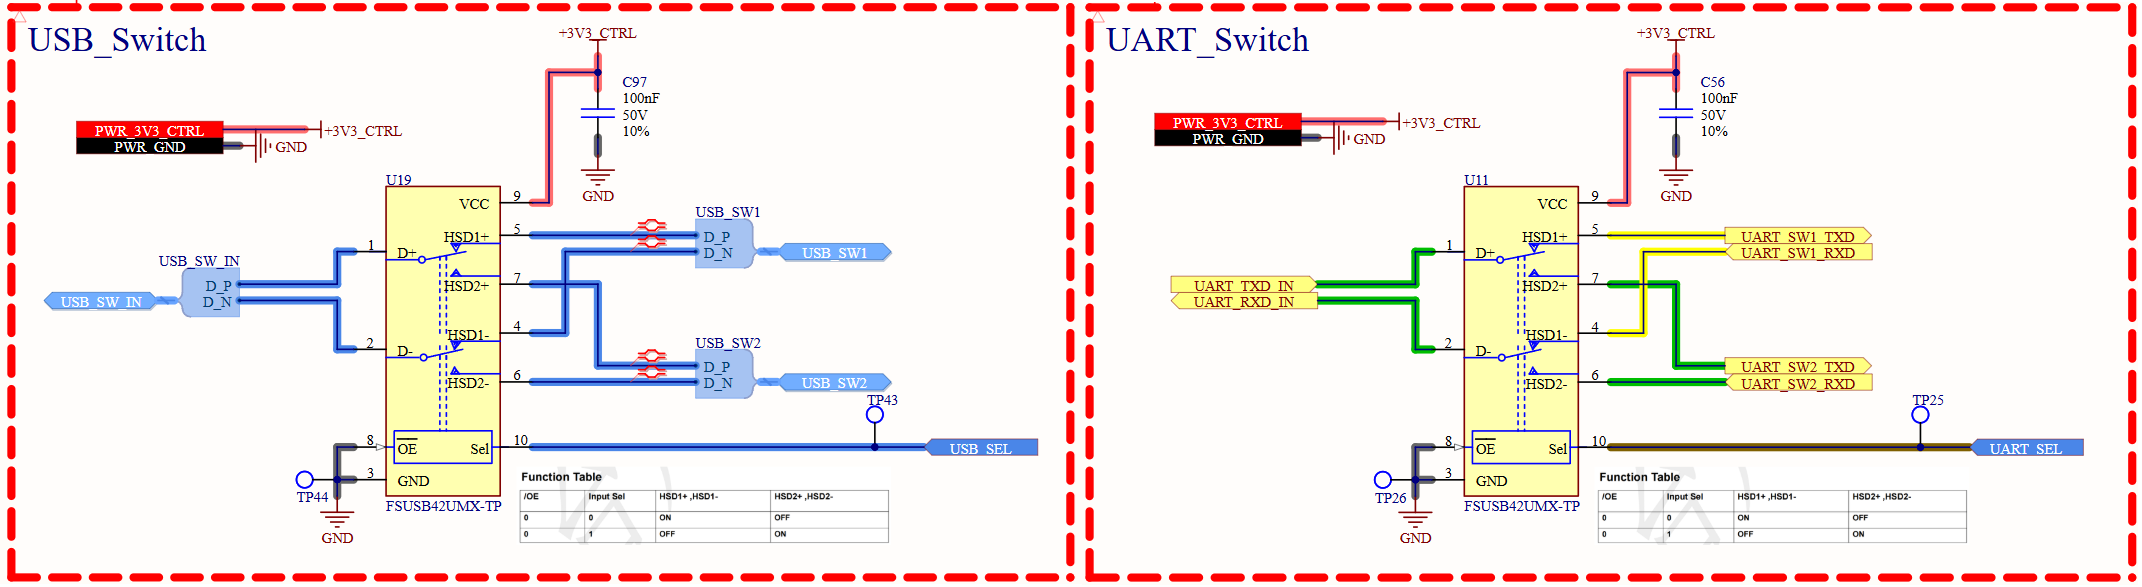
\includegraphics[width=\textwidth]{figures/DATN/sche_usb-uart_switch.png}
                \caption{Sơ đồ nguyên lý mạch USB/UART Switch} 
                \label{fig:sche_usb-uart_switch}
            \end{figure}

            Kiến trúc hệ thống tối ưu hóa cổng UART2 cho cả nhiệm vụ nạp firmware Slave và giao tiếp HMI, giúp tiết kiệm tối đa tài nguyên phần cứng. Nhằm xử lý triệt để sự chênh lệch điện áp logic giữa MCU (3.3V) và màn hình (5V), thiết kế sử dụng IC TXS0102DQER làm giải pháp chuyển mức hai chiều chuyên dụng. Đây là lựa chọn kỹ thuật cần thiết để bảo vệ chủ động các chân I/O khỏi rủi ro quá áp, đồng thời đảm bảo tính chính xác và độ tin cậy của tín hiệu điều khiển trong suốt quá trình vận hành.
            \begin{figure}[H]
                \centering
                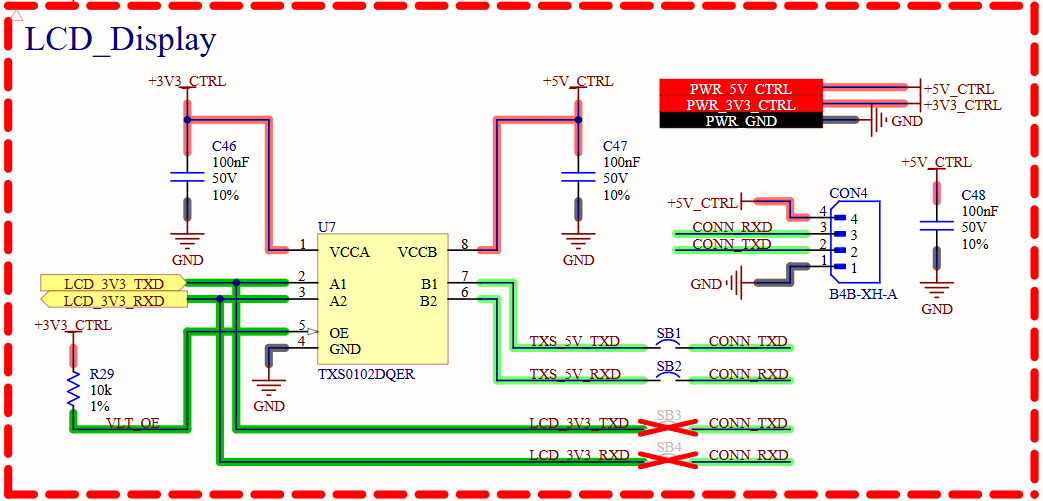
\includegraphics[width=0.75\textwidth]{figures/DATN/sche_lcd.png}
                \caption{Sơ đồ nguyên lý mạch LCD} 
                \label{fig:sche_lcd}
            \end{figure}
        
        \subsection{Thiết kế Mạch I\textsuperscript{2}C Buffer}   
            Để bảo đảm tính toàn vẹn dữ liệu khi giao tiếp với nhiều thiết bị ngoại vi qua dây dẫn dài, thiết kế tích hợp IC đệm TCA9803DGKR làm giải pháp phân tách bus chủ động. Lựa chọn này là kỹ thuật cần thiết để hệ thống vận hành ổn định ở chế độ Fast-mode (400kHz) mà không bị ảnh hưởng bởi giới hạn điện dung ký sinh 400pF. Việc sử dụng IC đệm giúp cô lập tải chỉ còn 10pF cho bus chính, đồng thời duy trì khả năng truyền dẫn tin cậy cho các nhánh mở rộng, giảm thiểu rủi ro lỗi bit do nhiễu và suy hao tín hiệu.
            \begin{figure}[H]
                \centering
                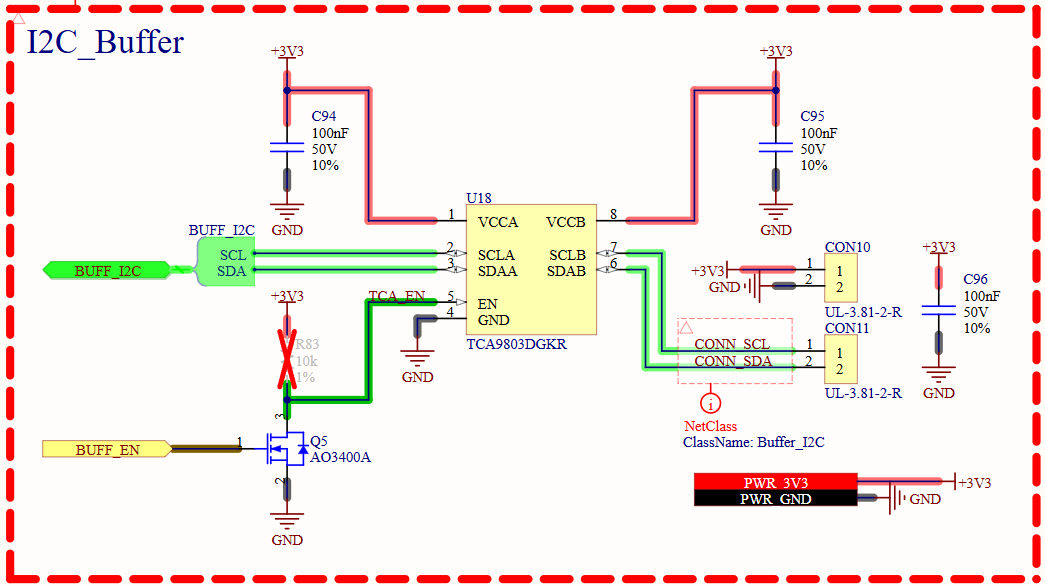
\includegraphics[width=0.75\textwidth]{figures/DATN/sche_i2cbuffer.png}
                \caption{Sơ đồ nguyên lý mạch I\textsuperscript{2}C Buffer} 
                \label{fig:sche_i2cbuffer}
            \end{figure}
        \subsection{Thiết kế Mạch nút nhấn}
            Thiết kế tích hợp diode TVS 3.3V để triệt tiêu chủ động xung ESD phát sinh từ tương tác cơ khí tại nút nhấn. Việc phối hợp tụ 100nF và trở giảm chấn 100\,$\Omega$ là giải pháp kỹ thuật cần thiết nhằm xử lý triệt để hiện tượng dội tiếp điểm (debounce) và ringing. Lựa chọn này đảm bảo tính toàn vẹn của tín hiệu truyền đến MCU, đồng thời tăng cường độ bền hệ thống trước các tác động điện-cơ trong điều kiện vận hành thực tế.
            \begin{figure}[H]
                \centering
                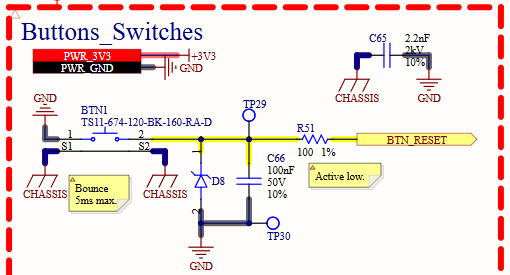
\includegraphics[width=0.75\textwidth]{figures/DATN/sche_button.png}
                \caption{Sơ đồ nguyên lý mạch nút nhấn} 
                \label{fig:sche_button}
            \end{figure}
        \subsection{Thiết kế Mạch điều khiển quạt DC}
            Quạt DC được tích hợp trong hệ thống nhằm phục vụ chức năng tản nhiệt trong quá trình vận hành. Nguồn cấp cho quạt được điều khiển thông qua một MOSFET kênh P, trong đó MCU master thực hiện điều khiển gián tiếp thông qua một transistor NPN tại cực G của MOSFET.

            \begin{figure}[H]
                \centering
                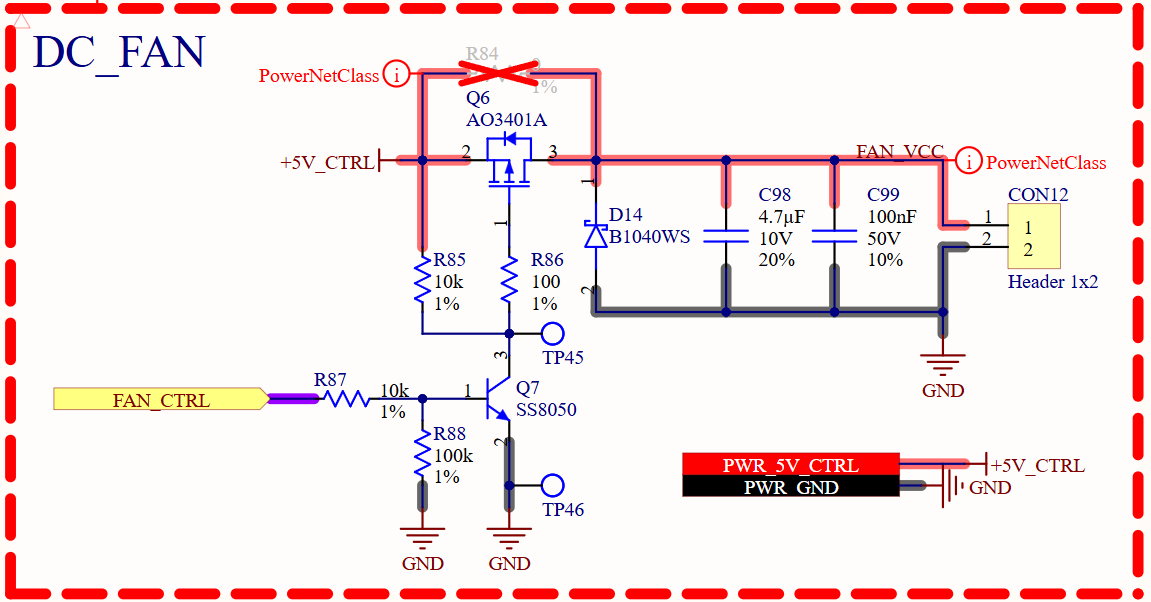
\includegraphics[width=0.7\textwidth]{figures/DATN/sche_dcfan.png}
                \caption{Sơ đồ nguyên lý mạch điều khiển quạt DC} 
                \label{fig:sche_dcfan}
            \end{figure}

            Ở trạng thái mặc định (không điều khiển), điện trở R88 kéo mức điện áp tại cực base của transistor NPN xuống thấp, khiến transistor không dẫn. Khi đó, điện trở R85 kéo cực G của MOSFET lên mức 3.3V, dẫn đến $V_{GS} = 0$, MOSFET tắt và quạt không hoạt động. Khi MCU đưa tín hiệu mức logic cao vào cực base của transistor NPN, transistor dẫn, kéo cực G của MOSFET xuống GND. Khi đó, $V_{GS} = -3.3V$, MOSFET được kích hoạt và cấp nguồn cho quạt, khiến quạt hoạt động.

            \begin{figure}[H]
                \centering
                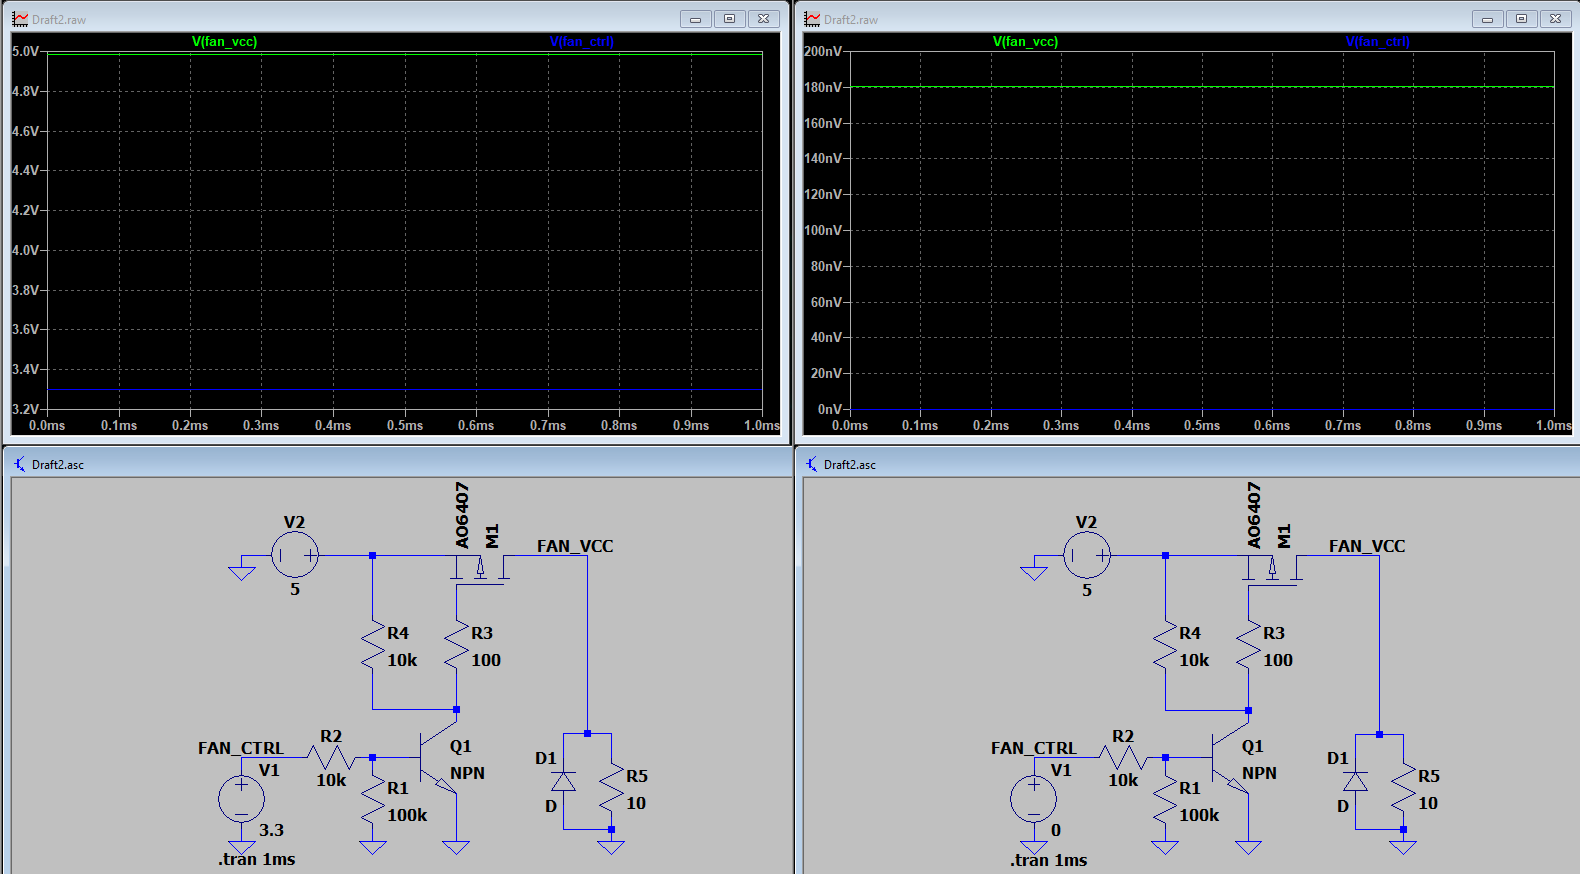
\includegraphics[width=\textwidth]{figures/DATN/simu_fandc.png}
                \caption{Thực hiện mô phỏng mạch điều khiển quạt DC trên LTspice} 
                \label{fig:simu_fandc}
            \end{figure}
            
            Tại đầu vào nguồn của quạt DC, một diode được mắc song song nhằm bảo vệ mạch cấp nguồn. Khi nguồn bị ngắt hoặc xuất hiện các xung điện áp trên đường cấp, diode tạo đường dẫn cho dòng điện quá độ lưu thông, giúp hạn chế điện áp đột biến và giảm ảnh hưởng đến các linh kiện điều khiển.
            
        % Nội dung mục này đã được chuyển lên Chương 4, mục 4.3.2 (Thiết kế Mạch Module Adapter).

    \section{Thiết kế PCB Layout (PCB Layout Design)}
        \subsection{Thiết kế PCB Stack-up và Kiểm soát trở kháng (Impedance Control)}
            \begin{enumerate}
                \renewcommand{\labelenumi}{\alph{enumi}.}
                \item \textbf{Thiết kế Stack-up:}
                \begin{itemize}
                    \item \textbf{Lựa chọn cấu trúc lớp:} Hệ thống bao gồm nhiều khối chức năng với các kênh tín hiệu tốc độ cao và đa dạng ray nguồn (power rails). Để đáp ứng các yêu cầu nghiêm ngặt về tính toàn vẹn tín hiệu (Signal Integrity - SI), tính toàn vẹn nguồn (Power Integrity - PI) và tương thích điện từ (EMC), thiết kế sử dụng cấu trúc PCB 6 lớp (6-layer stack-up) với sự phân bổ chức năng như sau:
                    
                    \begin{longtable}{|c|l|p{8cm}|}
                        \hline
                        \textbf{Lớp} & \textbf{Chức năng chính} & \textbf{Mô tả chi tiết} \\\hline
                        \endfirsthead
                        \hline
                        \textbf{Lớp} & \textbf{Chức năng chính} & \textbf{Mô tả chi tiết} \\\hline
                        \endhead
                        \hline
                        \endfoot
                        \endlastfoot  
                        
                        \textbf{L1} & Top Signal \& Power & Định tuyến tín hiệu tốc độ cao (High-speed), linh kiện SMD và các đường nguồn cục bộ. \\\hline
                        \textbf{L2} & Ground Plane & Mặt phẳng đất tham chiếu (Reference Plane) liên tục cho tín hiệu ở L1, giúp giảm diện tích vòng lặp và chắn nhiễu. \\\hline
                        \textbf{L3} & Power Plane & Mặt phẳng nguồn chính, phân phối năng lượng cho toàn bộ hệ thống. \\\hline
                        \textbf{L4} & Signal (Low-speed) & Định tuyến các tín hiệu tốc độ thấp, tín hiệu điều khiển hoặc các đường mạch không yêu cầu kiểm soát trở kháng khắt khe. \\\hline
                        \textbf{L5} & Ground Plane & Mặt phẳng đất tham chiếu liên tục cho tín hiệu ở L6. \\\hline
                        \textbf{L6} & Bottom Signal \& Power & Định tuyến tín hiệu tốc độ cao, linh kiện mặt dưới và đường nguồn phụ trợ. \\\hline
                    \end{longtable}

                    \begin{figure}[h]
                        \centering
                        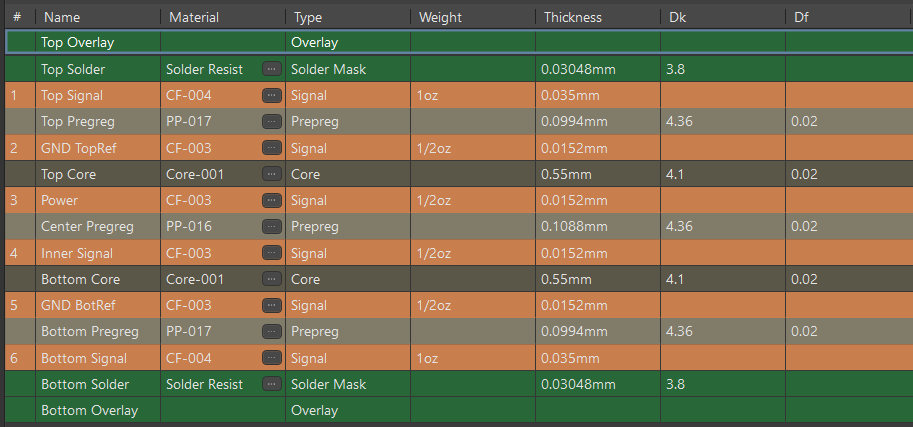
\includegraphics[width=0.75\textwidth]{figures/PCB_design_stackup.png}
                        \caption{Layer Stack-up Management}
                    \end{figure}
                \end{itemize}

                \item \textbf{Kiểm soát trở kháng (Impedance Control):}

                    \begin{figure}[h]
                        \centering
                        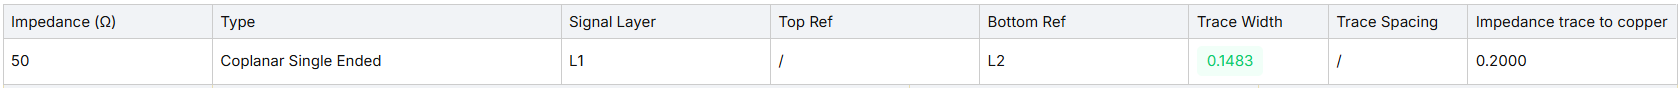
\includegraphics[width=\textwidth]{figures/impedance_50R.png}
                        \caption{Thông số kích thước cho đường tín hiệu Coplanar Single-ended $50\Omega$ (Đơn vị: mm)}
                    \end{figure}

                    \begin{figure}[h]
                        \centering
                        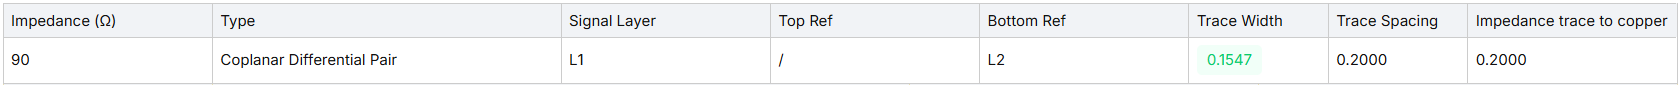
\includegraphics[width=\textwidth]{figures/impedance_90R.png}
                        \caption{Thông số kích thước cho cặp tín hiệu vi sai (Coplarar Differential-pair) $90\Omega$ (Đơn vị: mm)}
                    \end{figure}

                    \begin{figure}[h]
                        \centering
                        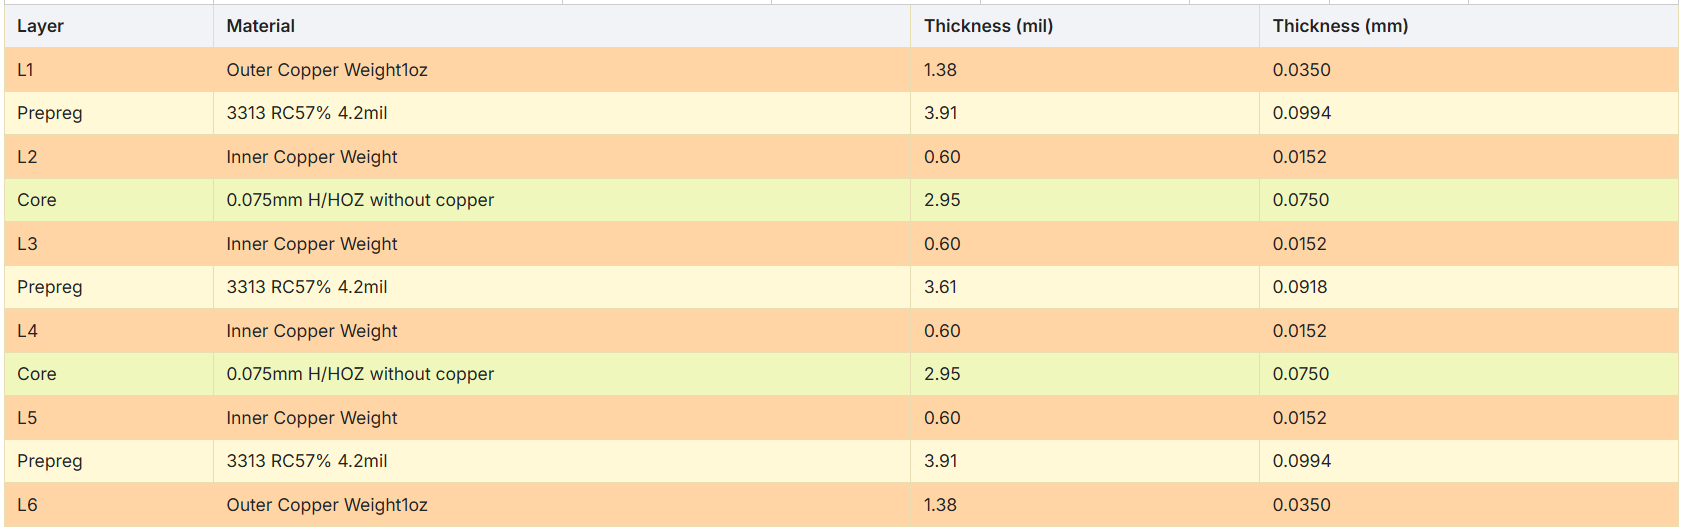
\includegraphics[width=0.75\textwidth]{figures/jlcpcb_stackup.png}
                        \caption{Cấu trúc Stack-up và thông số vật liệu tiêu chuẩn của JLCPCB}
                    \end{figure}
            \end{enumerate}
        \subsection{Quy hoạch và Bố trí linh kiện (Component Placement \& Floor-planning)}
            Việc bố trí linh kiện (Floor-planning) là bước quyết định đến hiệu năng chống nhiễu (EMC) và tính ổn định của hệ thống. Dựa trên sơ đồ nguyên lý và các ràng buộc cơ khí, chiến lược quy hoạch được thực hiện theo các nguyên tắc sau:

            \begin{enumerate}
                \renewcommand{\labelenumi}{\alph{enumi}.}
                \item \textbf{Phân vùng chức năng (Functional Partitioning):}
                \begin{itemize}
                    \item Bo mạch được chia thành các vùng chức năng vật lý riêng biệt dựa trên mức năng lượng và loại tín hiệu để giảm thiểu nhiễu giao thoa. Cụ thể bao gồm:
                    \begin{itemize}
                        \item \textbf{Vùng Nguồn (Power Zone):} Bố trí cục bộ gần đầu vào DC để cô lập nhiễu chuyển mạch.
                        \item \textbf{Vùng Xử lý trung tâm (Digital Core):} Chứa MCU Master và Slave, đặt tại trung tâm để tối ưu hóa đường đi tín hiệu.
                        \item \textbf{Vùng Giao tiếp Modular (Interface Zone):} Bố trí dọc theo các cạnh bo mạch để thuận tiện cho thao tác cắm rút module.
                        \item \textbf{Vùng RF (RF Zone):} Dành riêng cho các module không dây và anten.
                    \end{itemize}
                \end{itemize}
            % \begin{figure}[h]
            %     \centering
            %     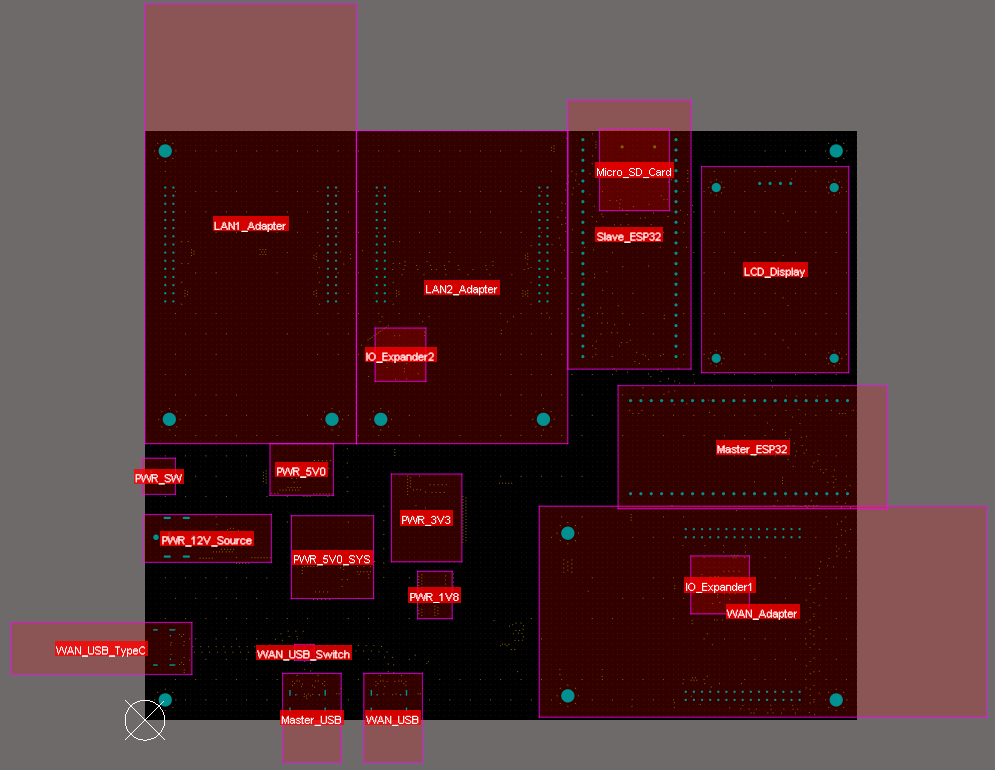
\includegraphics[width=0.45\textwidth]{figures/floor_planing.png} 
            %     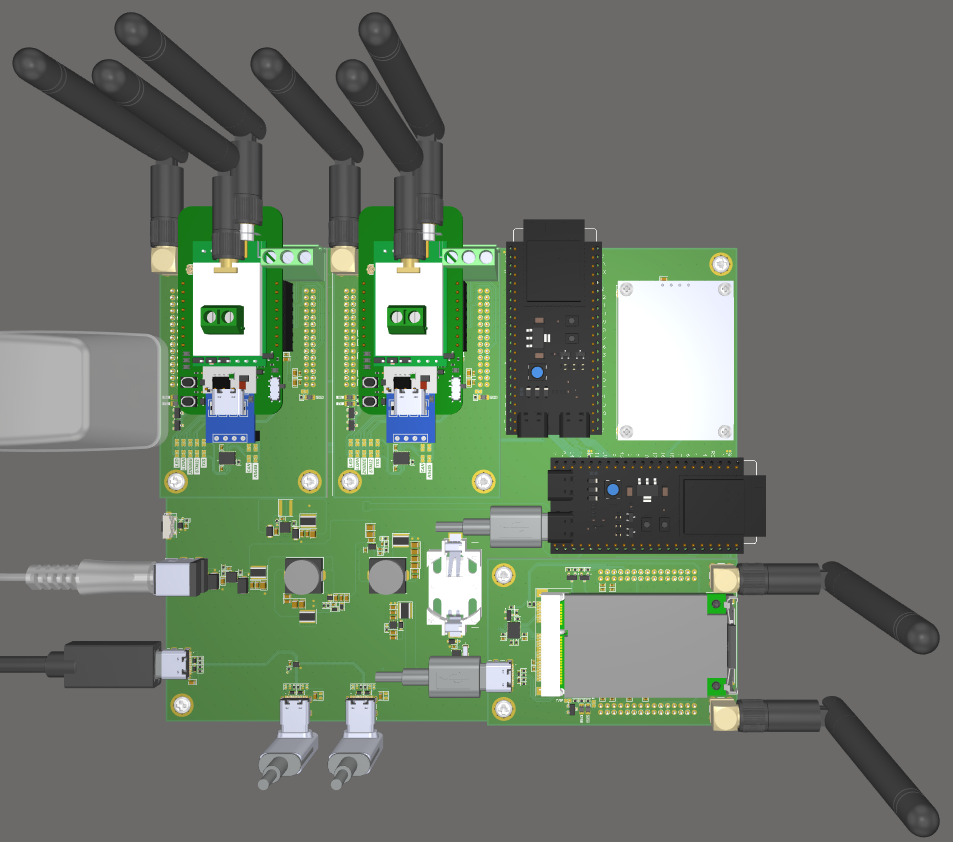
\includegraphics[width=0.45\textwidth]{figures/floor_planing_3d.png} 
            %     \caption{Sơ đồ quy hoạch phân vùng chức năng trên PCB (Floor-planning)}
            %     \label{fig:pcb_floorplan}
            % \end{figure}
            \begin{figure}[h]
                \centering
                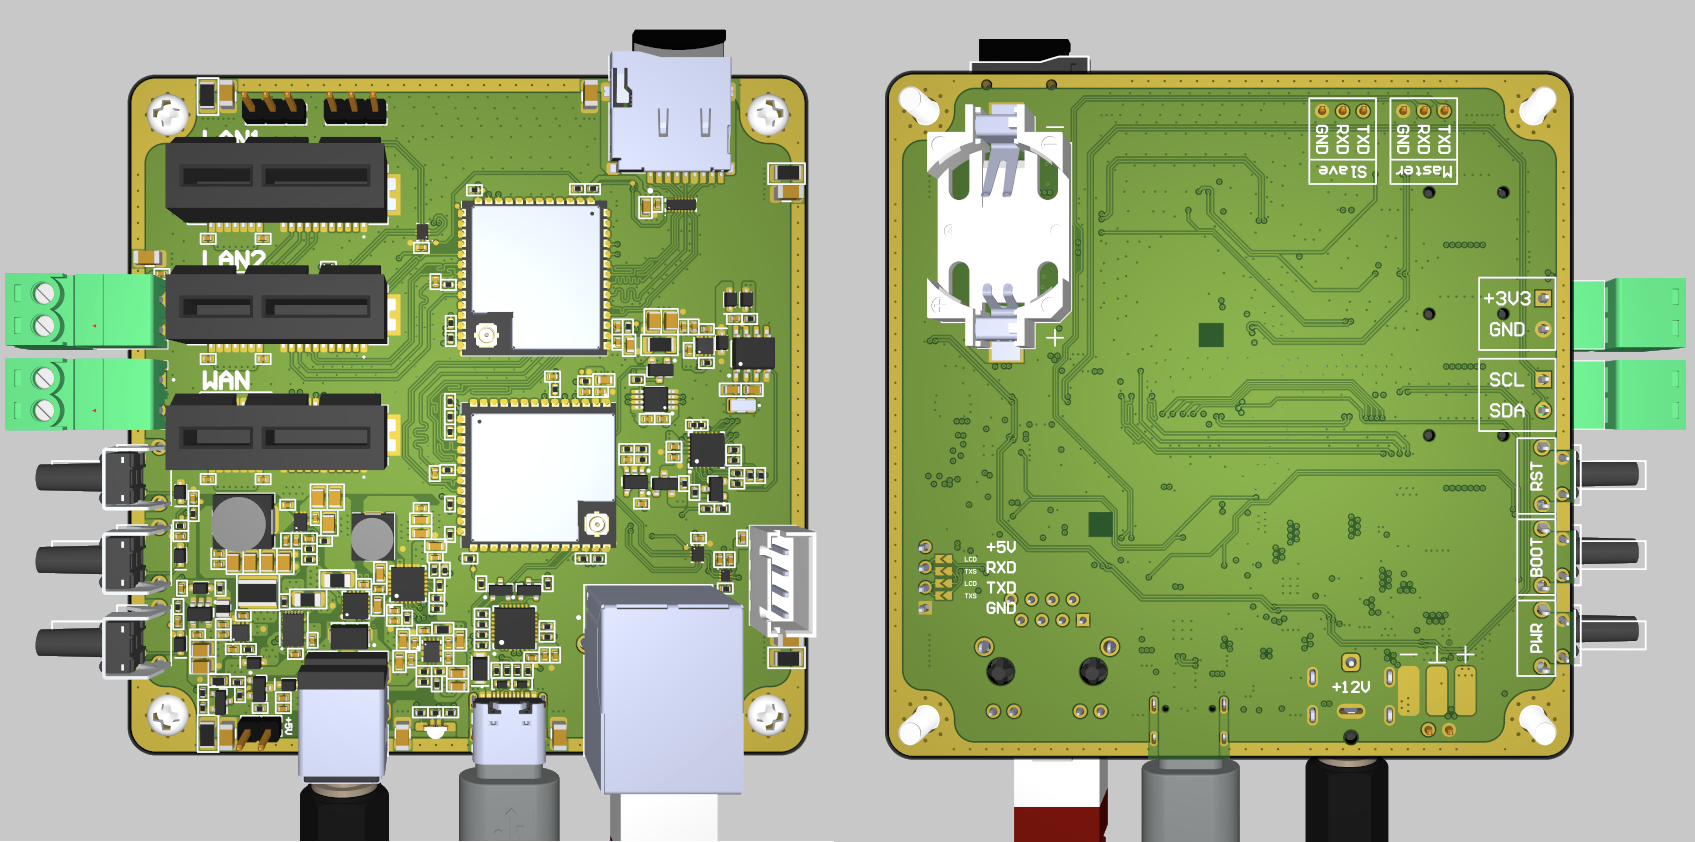
\includegraphics[width=0.75\textwidth]{figures/DATN/floor_planing_3d.png} 
                \caption{Sơ đồ quy hoạch phân vùng chức năng trên PCB (Floor-planning).}
                \label{fig:pcb_floorplan}
            \end{figure}

                \item \textbf{Tối ưu hóa Luồng tín hiệu (Signal Flow Optimization):}
                \begin{itemize}
                    \item \textbf{Vị trí vi xử lý:} Hai MCU được đặt sát nhau và đặt ở vị trí phù hợp so với các Module Adapter xung quanh. Điều này giúp cân bằng và giảm thiểu chiều dài đường mạch đến các cổng kết nối xung quanh, đặc biệt quan trọng với các bus giao tiếp tốc độ cao như Quad-SPI và các đường điều khiển tới Module Adapter.
                    \item \textbf{Tín hiệu tốc độ cao:} Các linh kiện liên quan đến giao tiếp tốc độ cao (như USB Switch, ESD protection) được đặt thẳng hàng và sát nhất có thể với cổng kết nối vật lý. Mục tiêu là giảm thiểu chiều dài đường dây (Trace length), từ đó giảm cảm kháng ký sinh và suy hao tín hiệu.
                \end{itemize}

                \item \textbf{Kiểm soát Nhiễu điện từ (EMI Management):}
                \begin{itemize}
                    \item \textbf{Cách ly nguồn nhiễu:} Các thành phần gây nhiễu mạnh như mạch nguồn xung (Buck Converter), cuộn cảm, và diode chuyển mạch được quy hoạch xa khỏi các khu vực nhạy cảm như khối Analog, mạch tạo dao động (Crystal Oscillator) và khối RF.
                    \item \textbf{Phân tách không gian RF:} Các vị trí dành cho module RF (như WiFi, LoRa) được bố trí tại các góc hoặc rìa của bo mạch. Khoảng cách vật lý giữa các anten được tối đa hóa (Spatial Diversity) và đặt chéo góc nhau để giảm hiện tượng bão hòa đầu vào hoặc giao thoa sóng vô tuyến (Co-existence interference).
                \end{itemize}

                \item \textbf{Tương thích Cơ khí và Sản xuất (DFM/DFA):}
                \begin{itemize}
                    \item \textbf{Giao diện kết nối:} Các thành phần tương tác với người dùng (Cổng USB, Khe thẻ nhớ, Nút nhấn, Đèn LED) được bố trí tại các mép bo mạch (Edge Placement), tuân thủ các ràng buộc về vị trí đảm bảo khả năng thao tác kết nối.
                    \item \textbf{Vùng cấm (Keep-out Zone):} Thiết lập các vùng cấm đi dây và đặt linh kiện xung quanh các lỗ bắt vít (Mounting holes) và khu vực anten PCB để tránh chập mạch hoặc ảnh hưởng đến bức xạ sóng.
                \end{itemize}
            \end{enumerate}

        \subsection{Kỹ thuật Chống nhiễu và Giảm thiểu EMI}
            Để đảm bảo thiết bị hoạt động ổn định trong môi trường công nghiệp và tuân thủ các tiêu chuẩn về tương thích điện từ (EMC), thiết kế PCB áp dụng các kỹ thuật layout sau:

            \begin{enumerate}
                \renewcommand{\labelenumi}{\alph{enumi}.}
                \item \textbf{Kỹ thuật Che chắn và Lồng Faraday:}
                \begin{itemize}
                    \item \textbf{Phủ mass toàn mạch:} Các diện tích trống trên tất cả các lớp PCB đều được phủ đồng nối đất (GND). Việc này tạo ra một lồng chắn tĩnh điện tự nhiên, giúp hấp thụ các nhiễu bức xạ từ môi trường và giảm thiểu phát xạ từ các đường mạch nội bộ.
                    \item \textbf{Vòng bảo vệ và Via Stitching:} Đối với các khu vực nhạy cảm hoặc nguồn gây nhiễu mạnh như mạch dao động thạch anh (Crystal Oscillator) và cặp dây vi sai USB tốc độ cao, kỹ thuật "khâu via" (Via Stitching) được áp dụng. Các lỗ via nối đất được đặt bao quanh linh kiện/đường mạch với mật độ cao (khoảng cách $<\lambda/20$ tần số hoạt động). Cấu trúc này hoạt động như một bức tường chắn sóng (Shielding Wall), cô lập nhiễu điện từ lan truyền ngang qua lớp điện môi.
                \end{itemize}
                
                \begin{figure}[h]
                    \centering
                    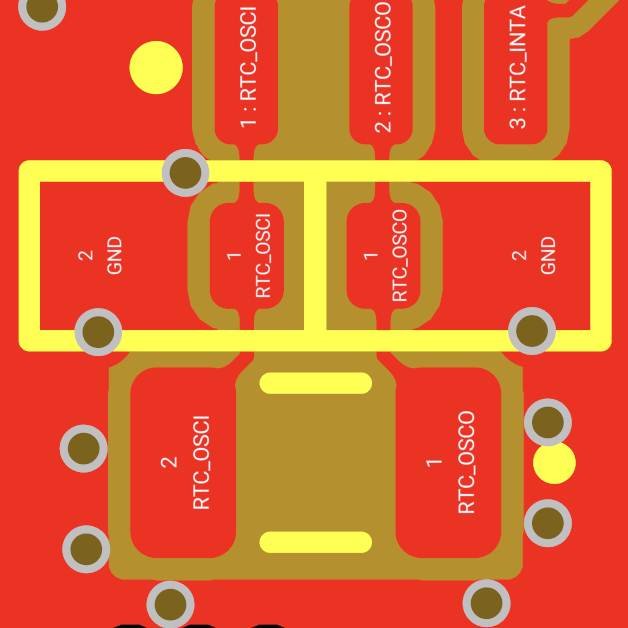
\includegraphics[width=0.375\textwidth]{figures/DATN/crysal_shielding_2D.png}
                    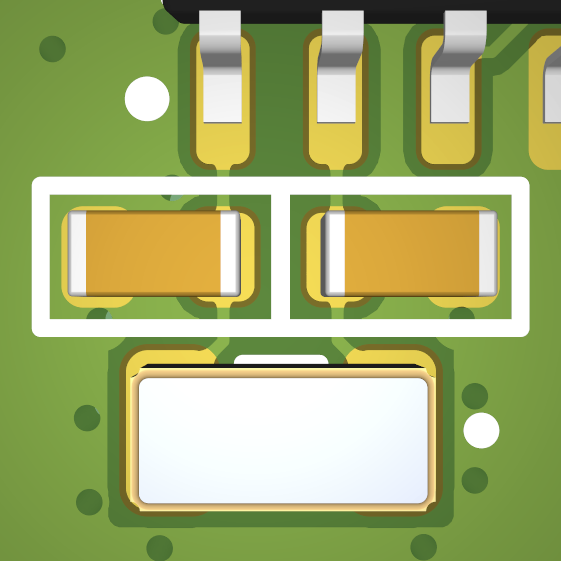
\includegraphics[width=0.375\textwidth]{figures/DATN/crysal_shielding_3D.png}
                    \caption{Kỹ thuật tạo Guard Ring và via stitching xung quanh khối thạch anh để cô lập nhiễu.}
                    \label{fig:crystal_shielding}
                \end{figure}

                \begin{figure}[h]
                    \centering
                    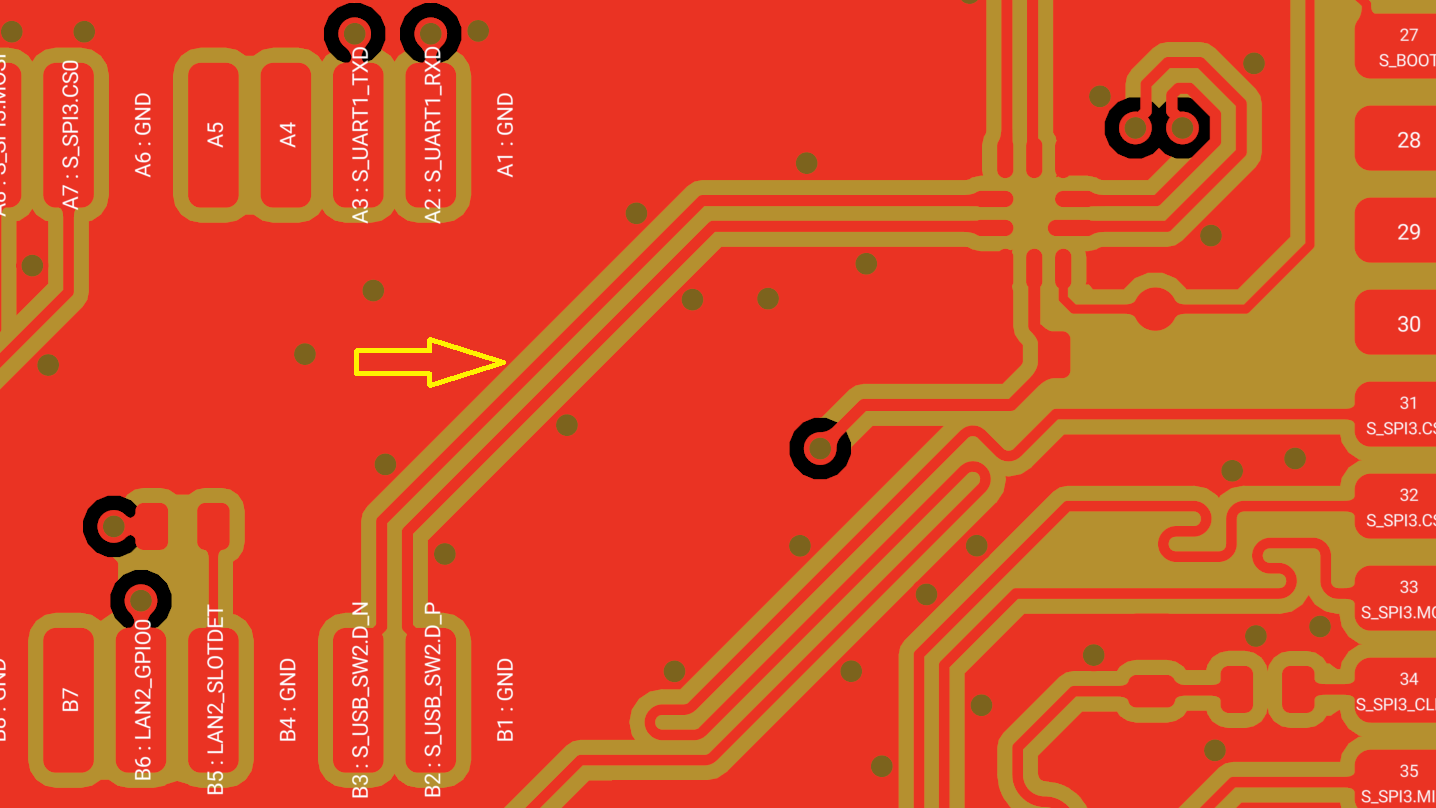
\includegraphics[width=0.75\textwidth]{figures/DATN/USB_shielding_2D.png}
                    \caption{Kỹ thuật bọc mass và stitching via dọc theo đường tín hiệu USB tốc độ cao.}
                    \label{fig:usb_shielding}
                \end{figure}

                \item \textbf{Quản lý Đường hồi tiếp tín hiệu:}
                \begin{itemize}
                    \item \textbf{Nguyên lý đường dẫn cảm kháng thấp nhất:} Ở tần số cao, dòng điện hồi tiếp luôn có xu hướng chạy ngay bên dưới đường dây tín hiệu trên mặt phẳng tham chiếu (Reference Plane) để tối thiểu hóa cảm kháng vòng lặp.
                    \item \textbf{Tránh cắt xẻ mặt phẳng đất:} Thiết kế đảm bảo các mặt phẳng đất (L2, L5) là liên tục và liền mạch. Tuyệt đối tránh đi dây tín hiệu tốc độ cao cắt ngang qua các khe hở (Splits) hoặc vùng trống (Voids) trên lớp đất. Việc tín hiệu băng qua khe hở sẽ buộc dòng hồi tiếp phải đi vòng xa hơn, tạo thành một vòng lặp diện tích lớn (Large Loop Area). Vòng lặp này hoạt động như một anten khung (Loop Antenna), vừa phát xạ nhiễu ra ngoài vừa thu nhiễu từ môi trường vào, gây suy giảm chất lượng tín hiệu.
                \end{itemize}
                
                \begin{figure}[h]
                    \centering
                    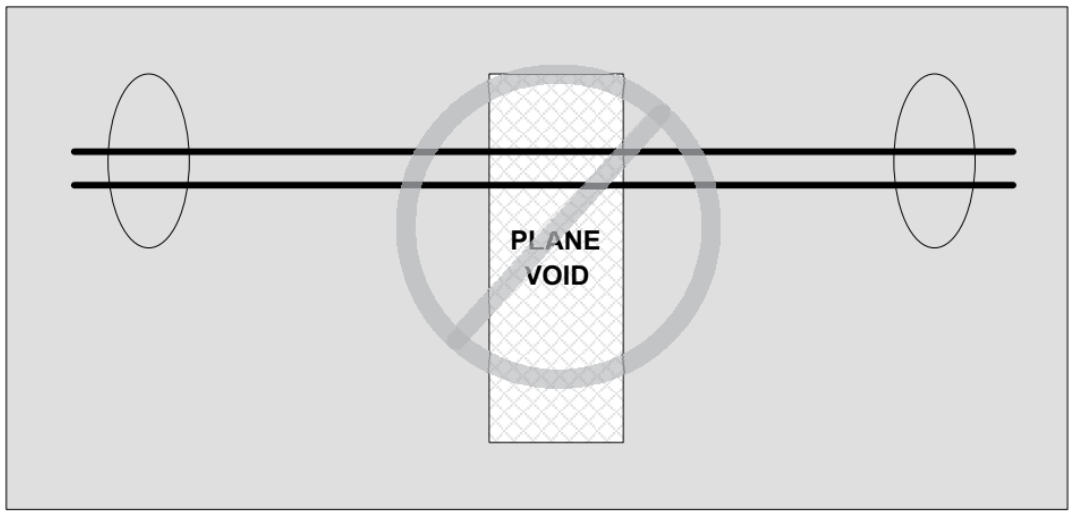
\includegraphics[width=0.48\textwidth]{figures/incorrect_plane_void_routing.png}
                    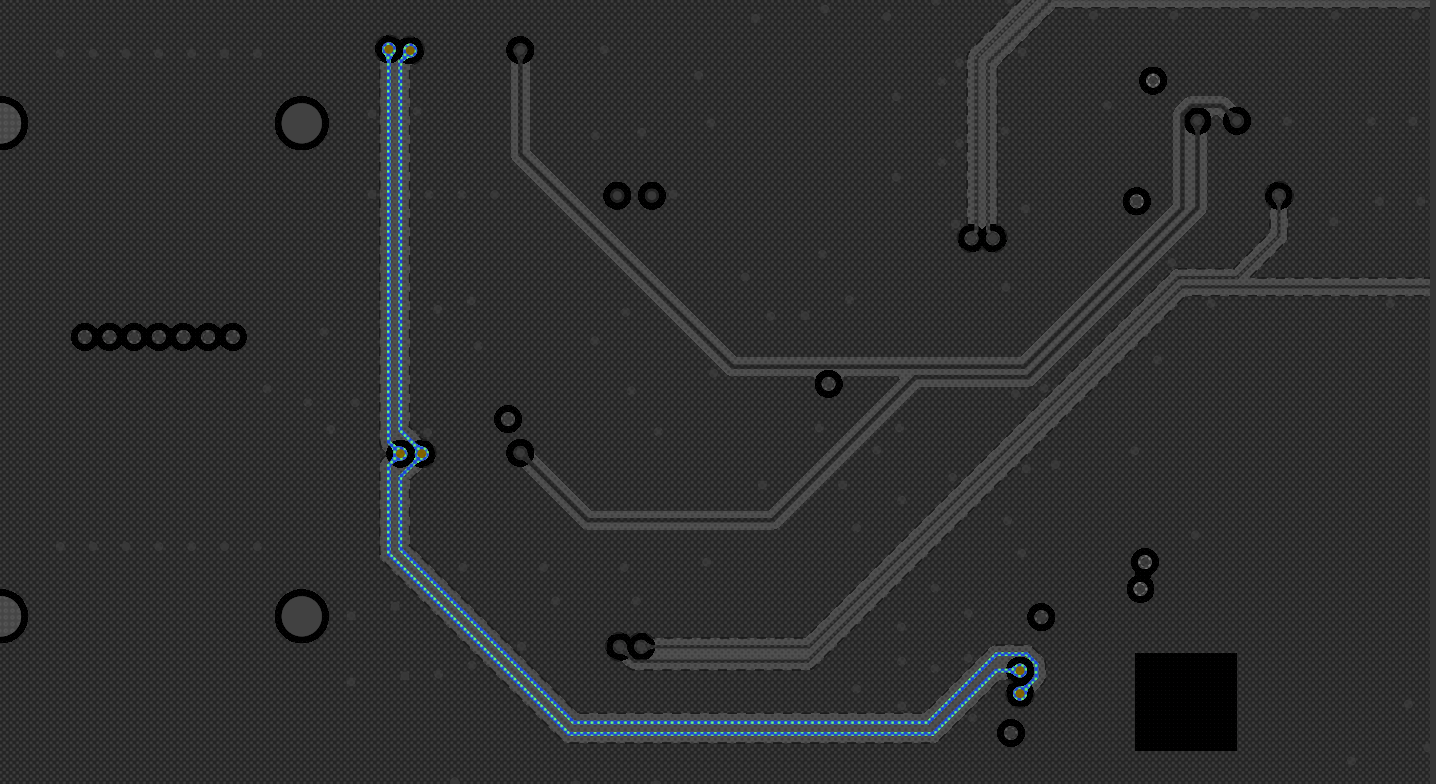
\includegraphics[width=0.48\textwidth]{figures/DATN/slave_i2c0.png}
                    \caption{Tín hiệu Slave\_I2C0 được định tuyến liên tục trên mặt phẳng GND đồng nhất.}
                \end{figure}

            \end{enumerate}

        \subsection{Kỹ thuật Layout Hệ thống Nguồn và PDN}

            Hệ thống nguồn đóng vai trò then chốt trong việc đảm bảo độ ổn định cho toàn bộ thiết bị. Dựa trên các hướng dẫn thiết kế (Design Guidelines) từ nhà sản xuất IC và nguyên lý điện từ trường, quy trình layout tuân thủ các nguyên tắc nghiêm ngặt sau:

            \begin{enumerate}
                \renewcommand{\labelenumi}{\alph{enumi}.}

                \begin{figure}[H]
                    \begin{minipage}{0.3\textwidth}
                        \centering
                        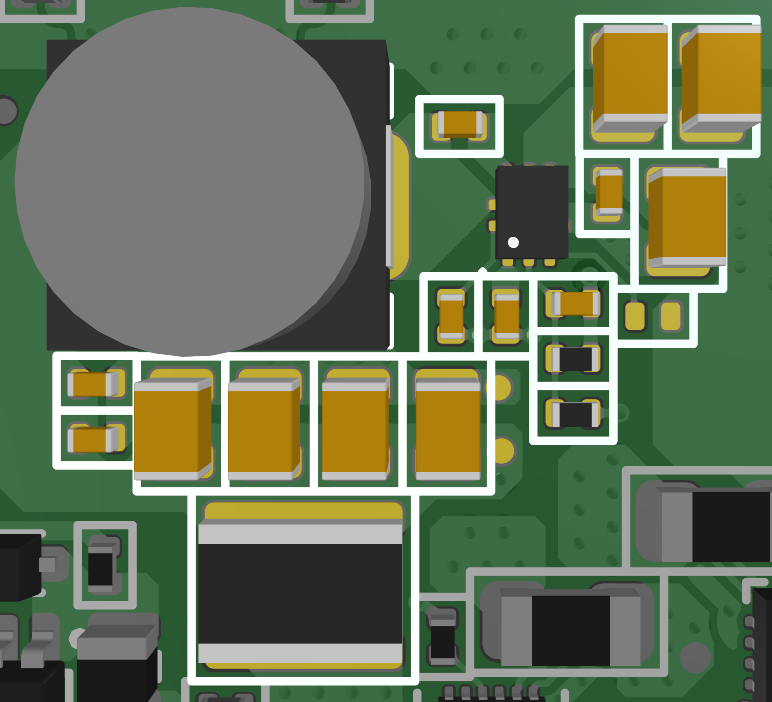
\includegraphics[width=\textwidth]{figures/hot_loop_minimization.png}
                        \caption{Vị trí các tụ điện trong nguồn xung +3V3.}
                    \end{minipage}
                    \hfill
                    \begin{minipage}{0.65\textwidth}
                        \item \textbf{Tối ưu hóa Vòng lặp Dòng điện (Hot Loop):}
                        \begin{itemize}
                            \item Các tụ điện đầu vào ($C_{IN}$) và đầu ra ($C_{OUT}$) là nguồn cung cấp năng lượng tức thời cho bộ chuyển đổi. Chúng được bố trí sát nhất có thể với các chân $V_{IN}/GND$ và $V_{OUT}/PGND$ của IC nguồn hoặc cuộn cảm cho nguồn xung.
                            \item Mục tiêu là giảm thiểu diện tích vật lý của "vòng lặp xung" (Hot Loop Area) - nơi có dòng điện biến thiên $di/dt$ lớn nhất. Việc này giúp giảm cảm kháng ký sinh đường dây, hạn chế các xung gai điện áp (Voltage Spikes) và giảm thiểu bức xạ nhiễu EMI ra môi trường.
                        \end{itemize}
                    \end{minipage}
                \end{figure}
                \begin{figure}[H]
                    \begin{minipage}{0.65\textwidth}
                        \item \textbf{Xử lý Điểm chuyển mạch (Switching Node):}
                        \begin{itemize}
                            \item Chân SW (Switching) là nơi dao động điện áp tần số cao với biên độ lớn ($dv/dt$ cao). Đường mạch tại đây được thiết kế dạng khối đồng (Polygon) ngắn và rộng để giảm điện trở và cảm kháng, nhưng diện tích không được quá lớn để hạn chế điện dung ký sinh gây tổn hao.
                            \item Thiết kế đảm bảo tuyệt đối không định tuyến bất kỳ đường tín hiệu nhạy cảm nào đi ngang qua hoặc đi ở lớp ngay bên dưới (Layer 2) của cuộn cảm và điểm SW để tránh nhiễu.
                        \end{itemize}
                    \end{minipage}
                    \hfill
                    \begin{minipage}{0.3\textwidth}
                        \centering
                        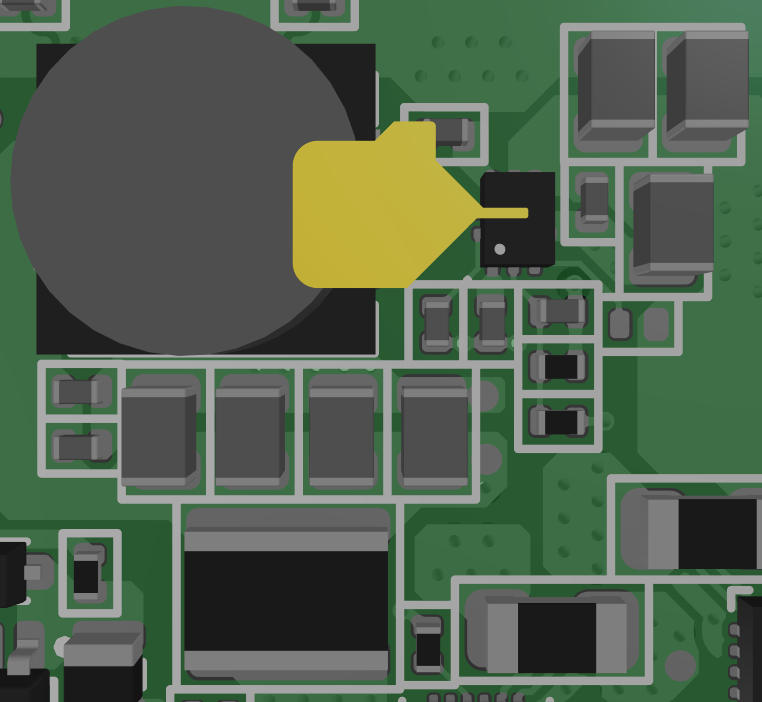
\includegraphics[width=\textwidth]{figures/switching_node.png}
                        \caption{Điểm chuyển mạch trong nguồn xung +3V3.}
                    \end{minipage}
                \end{figure}
                \begin{figure}[H]
                    \begin{minipage}{0.3\textwidth}
                        \centering
                        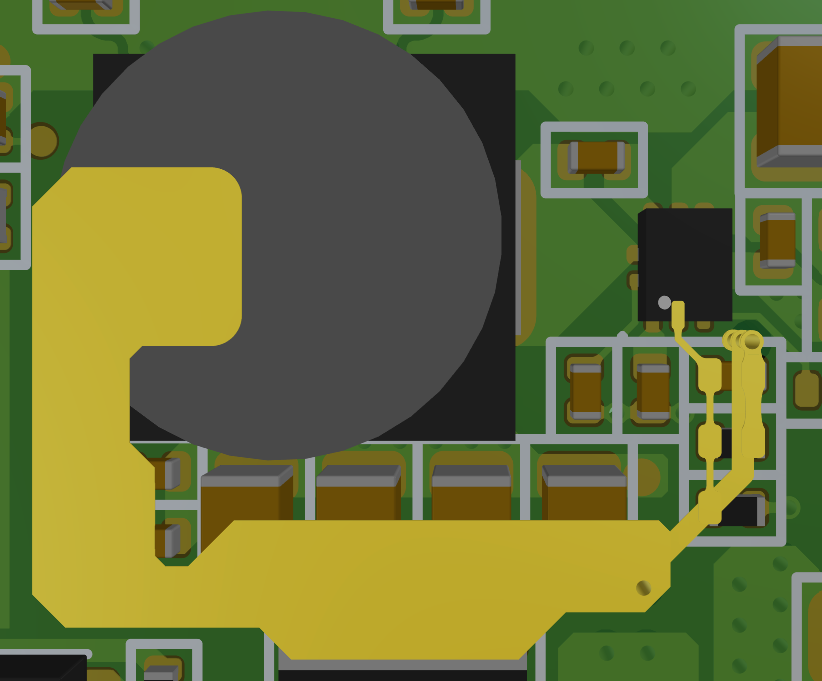
\includegraphics[width=\textwidth]{figures/feedback.png}
                        \caption{Định tuyến hồi tiếp trong nguồn xung +3V3.}
                    \end{minipage}
                    \hfill
                    \begin{minipage}{0.65\textwidth}
                        \item \textbf{Kỹ thuật Hồi tiếp (Feedback) và Ground:}
                        \begin{itemize}
                            \item \textbf{Kết nối Kelvin:} Đường tín hiệu hồi tiếp (Feedback) được lấy mẫu trực tiếp tại điểm sau tụ đầu ra $C_{OUT}$ để đảm bảo điện áp đo được là chính xác nhất.
                            \item \textbf{Cách ly nhiễu:} Đường Feedback được đi tránh xa khỏi cuộn cảm và điểm SW. Ground của đường hồi tiếp và các linh kiện tín hiệu nhỏ (như tụ Soft-start, trở định thời) được nối vào Analog Ground (AGND) hoặc chân GND tín hiệu của IC, tách biệt với Power Ground (PGND) đang chịu dòng xung lớn, nhằm tránh nhiễu mặt đất (Ground Bounce).
                        \end{itemize}
                    \end{minipage}
                \end{figure}
                \item \textbf{Quản lý Nhiệt (Thermal):}
                \begin{itemize}
                    \item Tận dụng Pad tản nhiệt dưới bụng IC, thiết kế sử dụng mảng via tản nhiệt dày đặc để dẫn nhiệt trực tiếp xuống các lớp đồng Ground Plane rộng lớn ở bên dưới (L2, L5). Điều này biến toàn bộ bo mạch thành một lá tản nhiệt tự nhiên, đảm bảo IC hoạt động mát mẻ dưới tải dòng lớn.
                \end{itemize}

                % \newpage
                \begin{figure}[H]
                        \begin{minipage}{0.3\textwidth}
                        \centering
                        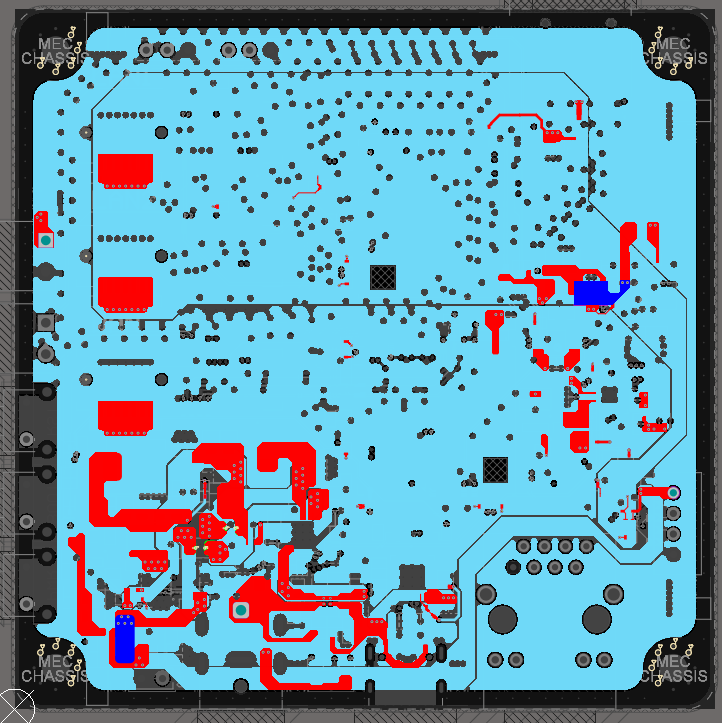
\includegraphics[width=\textwidth]{figures/power_network.png}
                        \caption{Mạng phân phối nguồn.}
                    \end{minipage}
                    \hfill
                    \begin{minipage}{0.65\textwidth}
                        \item \textbf{Thiết kế Mạng phân phối nguồn (Power Distribution Network - PDN):}
                        Mục tiêu cốt lõi là duy trì trở kháng nguồn ($Z_{PDN}$) thấp hơn trở kháng mục tiêu trên toàn dải tần số hoạt động. Chiến lược thực hiện bao gồm:
                        \begin{itemize}
                            \item \textbf{Tụ điện phẳng:} Trong cấu trúc Stack-up 6 lớp, việc bố trí Lớp 2 (Ground) và Lớp 3 (Power) liền kề nhau với lớp cách điện mỏng tạo ra một tụ điện ký sinh lớn, giúp lọc các nhiễu tần số cực cao mà tụ điện rời không đáp ứng kịp.
                            \item \textbf{Tụ điện Decoupling đa tầng:} Sử dụng tổ hợp nhiều giá trị tụ điện song song. Các tụ giá trị nhỏ (10pF - 100nF) đặt sát chân cấp nguồn của IC để triệt tiêu nhiễu cao tần/xung nhịp MCU. Các tụ giá trị lớn (10$\mu$F - 100$\mu$F) đặt gần đó để đáp ứng nhu cầu năng lượng cho các biến động tải lớn.
                        \end{itemize}
                    \end{minipage}
                \end{figure}     

                \begin{itemize}
                    \item \textbf{Hình dạng đường dây:} 
                    \begin{itemize}
                        \item Các đường dẫn nguồn chính được thiết kế dạng mặt phẳng (Plane) hoặc đường mạch rất rộng. Theo công thức $L \propto \ln(1/W)$, đường mạch càng rộng thì cảm kháng ký sinh ($L$) càng nhỏ.
                        \item Việc giảm cảm kháng $L$ giúp hạn chế hiện tượng sụt áp quá độ ($V_{drop} = L \cdot di/dt$) khi tải thay đổi đột ngột và giảm thiểu hiện tượng đổ chuông (Ringing) gây mất ổn định điện áp. Đồng thời, tiết diện dây lớn giúp giảm mật độ dòng điện, giảm tỏa nhiệt trên đường dây (IR Loss).
                    \end{itemize}   
                \end{itemize}      
            \end{enumerate}
            \newpage

        \subsection{Kỹ thuật Định tuyến Tín hiệu Tốc độ cao (High-Speed Signal Routing)}

            Để đảm bảo chất lượng tín hiệu (Signal Integrity) cho các giao tiếp USB, SPI và SDIO, quy trình layout tuân thủ các quy tắc định tuyến nghiêm ngặt nhằm kiểm soát trở kháng, đồng bộ pha và giảm thiểu xuyên nhiễu (Crosstalk):

            \begin{enumerate}
                \renewcommand{\labelenumi}{\alph{enumi}.}
                \item \textbf{Định tuyến Cặp Vi sai (Differential Pair Routing - USB):}
                \begin{itemize}
                    \item \textbf{Kiểm soát Trở kháng:} Cặp tín hiệu vi sai USB D+/D- được thiết kế đạt trở kháng đặc tính mục tiêu $Z_{diff} = 90\Omega \pm 10\%$. Cấu trúc định tuyến sử dụng là \textit{Differential Coplanar Waveguide} (vi sai đồng phẳng có mass bao bọc) để tăng khả năng chống nhiễu ngoại vi.
                    \item \textbf{Đồng bộ pha:} Đảm bảo chênh lệch chiều dài giữa hai dây P và N trong cùng một cặp là nhỏ nhất có thể tùy theo tốc độ truyền dữ liệu. Kỹ thuật \textit{Phase Matching} được thực hiện ngay tại điểm xảy ra lệch pha để đảm bảo tín hiệu đến bộ thu đồng thời, triệt tiêu nhiễu chế độ chung (Common Mode Noise).
                    \item \textbf{Tính đối xứng:} Hai đường dây được định tuyến song song và đối xứng tuyệt đối trong suốt chiều dài đường truyền. Các góc cua sử dụng góc vát $135^{\circ}$ hoặc cung tròn, tuyệt đối không dùng góc $90^{\circ}$ để tránh thay đổi trở kháng đột ngột.
                \end{itemize}

                \begin{figure}[h]
                    \centering
                    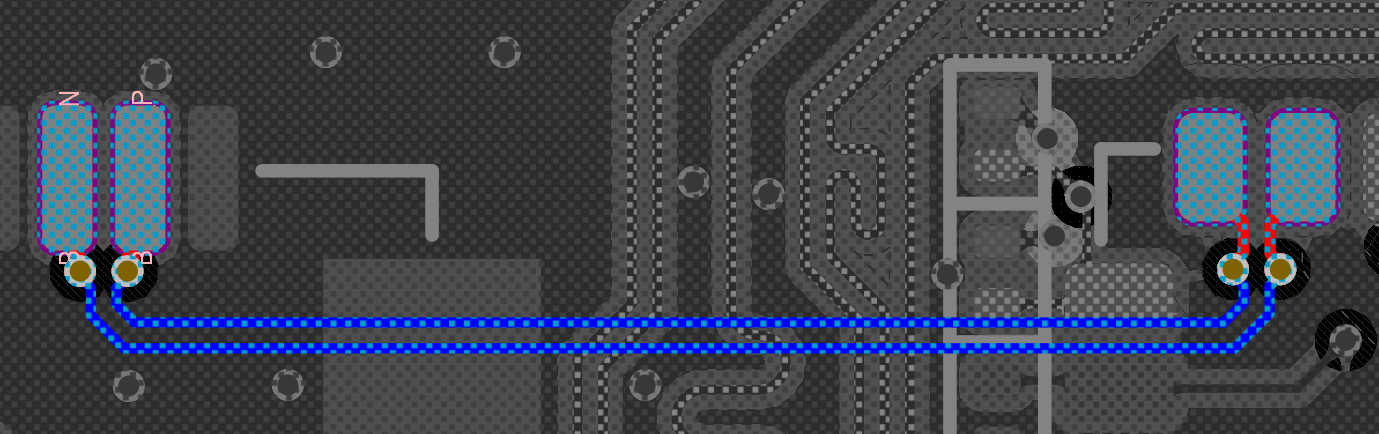
\includegraphics[width=0.5\textwidth]{figures/usb.png}
                    \caption{Định tuyến USB.}
                \end{figure} 

                % \newpage
                \item \textbf{Định tuyến Bus Đơn cực (Single-ended Bus Routing - SPI/SDIO):}
                \begin{itemize}
                    \item \textbf{Trở kháng $50\Omega$:} Tất cả các đường tín hiệu dữ liệu và điều khiển được thiết kế với trở kháng $Z_0 = 50\Omega \pm 10\%$ theo cấu trúc \textit{Coplanar Waveguide}.
                    \item \textbf{Bảo vệ xung nhịp (Clock Shielding):} Tín hiệu Clock (CLK) là nguồn gây nhiễu mạnh nhất. Đường CLK được định tuyến biệt lập, bao bọc bởi hai đường mass bảo vệ và được khâu via xuống Ground Plane dọc theo đường đi để cô lập trường điện từ.
                    \item \textbf{Cân bằng chiều dài (Trace Length Matching):} Áp dụng các kỹ thuật \textit{Accordion} và \textit{Trombone} để cân bằng chiều dài của các đường dữ liệu với đường Clock. Điều này đảm bảo dữ liệu được lấy mẫu chính xác tại sườn xung nhịp, tránh lỗi Setup/Hold time do độ trễ lan truyền (Propagation Delay).
                \end{itemize}
                
                % \newpage
                \item \textbf{Kiểm soát Nhiễu và Toàn vẹn tín hiệu (EMI \& SI Control):}
                \begin{itemize}
                    \item \textbf{Giảm thiểu Via:} Hạn chế tối đa việc chuyển lớp trên đường tín hiệu tốc độ cao để tránh gây gián đoạn trở kháng. Nếu bắt buộc phải chuyển lớp, các stitching via được đặt ngay cạnh via tín hiệu để duy trì đường hồi tiếp liền mạch.
                    \item \textbf{Định tuyến trực giao:} Để tránh hiện tượng xuyên nhiễu (Crosstalk) giữa các lớp liền kề được đi vuông góc với nhau. Tuyệt đối tránh đi dây song song chồng lên nhau.
                \end{itemize}
                \begin{figure}[H]
                    \begin{minipage}{0.3\textwidth}
                        \centering
                        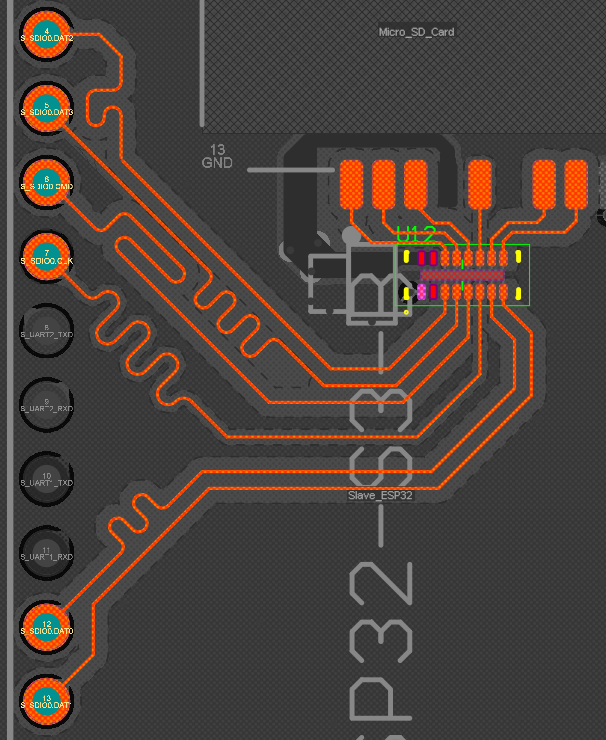
\includegraphics[width=\textwidth]{figures/sdio.png}
                        \caption{Định tuyến SDIO giữa ESP32-S3 Slave với Micro SD Card.}
                    \end{minipage}
                    \hfill
                    \begin{minipage}{0.65\textwidth}
                        \begin{itemize}
                            \item \textbf{Toàn vẹn mặt phẳng tham chiếu:} Tín hiệu tốc độ cao luôn được tham chiếu tới một mặt phẳng đất liền mạch (Solid Ground Plane). Tuyệt đối không định tuyến băng qua các khe hở (Splits) hoặc vùng trống (Voids) trên lớp đất để tránh làm gãy khúc đường hồi tiếp dòng điện.
                            \item \textbf{Quy tắc khoảng cách:} Áp dụng quy tắc 3W hoặc 5W (khoảng cách giữa các đường mạch lớn hơn 3-5 lần bề rộng đường dây) để giảm thiểu xuyên nhiễu giữa các bus tín hiệu khác nhau. Đồng thời, duy trì khoảng cách ly đối với các linh kiện gây nhiễu như thạch anh, cuộn cảm nguồn.
                        \end{itemize}
                    \end{minipage}
                \end{figure} 
            \end{enumerate}
